

\documentclass[authoryear,12pta4paper,fleqn]{article}


% \usepackage[paper=a4paper,top=1.5cm,left=1.2cm,right=0.8cm,
%     foot=1cm,bottom=1.5cm]{geometry}

\usepackage{arxiv}                  % https://www.overleaf.com/gallery/tagged/arxiv

\usepackage[utf8]{inputenc}         % utf8 support       %!!!!!!!!!!!!!!!!!!!!
\usepackage[T1]{fontenc} 
\usepackage{amsmath,amssymb, amsthm,mathtools,mathrsfs,stmaryrd,titletoc}


\usepackage{natbib}   % bibtex 
% need to install mtpro2
\let\Bbbk\relax
\usepackage[subscriptcorrection,slantedGreek,nofontinfo,mtphrd]{mtpro2}

\usepackage[retainorgcmds]{IEEEtrantools}
\usepackage[usenames]{color}
\usepackage{tabularx}
\usepackage{booktabs}
\usepackage[font=small,labelfont=md]{caption,subfig}
\usepackage{multirow}
\usepackage[bookmarks=true,colorlinks=true,linkcolor=blue,citecolor=red,backref=page]{hyperref}
\usepackage{float}         % make new float environment such as boxes (captioned)
\usepackage{listings}      % insert source code   
\usepackage{algorithm}
%\usepackage{algorithmicx}
\usepackage{algpseudocode}
\usepackage[most]{tcolorbox}
\usepackage{IEEEtrantools}
%\usepackage[ruled,vlined]{algorithm2e}
%\sloppy
%\usepackage{authblk}

% nomenclature and glossaries for XFEM, CDM
%\usepackage{nomencl}
\usepackage[acronym]{glossaries}

% the following packages just to improve the latex experience 
%\usepackage{silence} %
\usepackage{silence}
\WarningsOff
\usepackage{siunitx}
\usepackage[norefs,nocites,ignoreunlbld]{refcheck} % warning for unreferred figs/tables/equas
% search in the .log file for unused fig to detect figures not referred to in the text.
\usepackage[activate={true,nocompatibility},final,tracking=true,kerning=true,spacing=true,factor=1100,stretch=10,shrink=10]{microtype}
% activate={true,nocompatibility} - activate protrusion and expansion
% final - enable microtype; use "draft" to disable
% tracking=true, kerning=true, spacing=true - activate these techniques
% factor=1100 - add 10% to the protrusion amount (default is 1000)
% stretch=10, shrink=10 - reduce stretchability/shrinkability (default is 20/20)
\usepackage[capitalise]{cleveref} %Basically, cleveref must be loaded last.
% clever ref: instead of Fig.~\ref{d}, use \cref{d} or \Cref{d}  capitalise -> Figure 1
% \crefrange{eq1}{eq5}
\usepackage[textsize=tiny]{todonotes}
\usepackage{nicefrac} % type inline fractions: \nicefrac{1}{2}
\usepackage{setspace} % gives commands such as \doublespacing, or \begin{singlespace} \end{singlespace}
\usepackage{lineno}  % write numbers for lines
%\usepackage[mediumspace,mediumqspace,Grey,squaren]{SIunits}
%\usepackage{totcount} % to count the total number of references and other things
%\usepackage[figure,table]{totalcount}
\usepackage{blkarray, bigstrut} % write complicated matrices with borders, see http://mirror.lagoon.nc/pub/ctan/macros/latex/contrib/blkarray/blkarray.pdf
\usepackage{tikz}
\usetikzlibrary{arrows,decorations.pathmorphing,decorations.pathreplacing,backgrounds,positioning,fit,matrix,math,shapes.misc}
\tikzset{cross/.style={cross out, draw=black, minimum size=2*(#1-\pgflinewidth), inner sep=0pt, outer sep=0pt}, cross/.default={1pt}}
\usepackage{wasysym}
\usepackage{gensymb} % for degree symbol

\usepackage{pgfplots}
 \pgfplotsset{compat=newest}
 %% the following commands are needed for some matlab2tikz features
 \usetikzlibrary{plotmarks}
 \usetikzlibrary{arrows.meta}
 \usepgfplotslibrary{patchplots}
 \usepackage{grffile} % load graphicx package, The package extends the file name processing of package graphics to sup- port a larger range of file names. 
\usepackage{pgf}
%\usepackage{underscore}
\usepackage[english]{babel}  %also automatically activates the appropriate hyphenation rules for the language you choose
\usepackage[title,titletoc,toc]{appendix} 
%\usepackage[referable]{threeparttablex}
\usepackage{threeparttable}
\usepackage{xspace}
\usepackage[scaled=0.84]{beramono}
%\usepackage[breakwithin,symbol]{parnotes} % foonote in tables, but not good looking

%%%% these patches ensure that the backrefs point to the actual occurrences of the citations in the text, not just the page or section in which they appeared
%%%% https://tex.stackexchange.com/questions/54541/precise-back-reference-target-with-hyperref-and-backref
%%%% BEGIN BACKREF DIRECT PATCH, apply these AFTER loading hyperref package with appropriate backref option
% The following options are provided for the patch, currently with a poor interface!
% * If there are multiple cites on the same (page|section) (depending on backref mode),
%   should we show only the first one or should we show them all?
\newif\ifbackrefshowonlyfirst
\backrefshowonlyfirstfalse
%\backrefshowonlyfirsttrue
%%%% end of options
%
% hyperref is essential for this patch to make any sense, so it is not unreasonable to request it be loaded before applying the patch
\makeatletter
% 1. insert a phantomsection before every cite, so hyperref has something to target
%    * in case natbib is loaded. hyperref provides an appropriate hook so this should be safe, and we don't even need to check if natbib is loaded!
\let\BR@direct@old@hyper@natlinkstart\hyper@natlinkstart
\renewcommand*{\hyper@natlinkstart}{\phantomsection\BR@direct@old@hyper@natlinkstart}% note that the anchor will appear after any brackets at the start of the citation, but that's not really a big issue?
%    * if natbib isn't used, backref lets \@citex to \BR@citex during \AtBeginDocument
%      so just patch \BR@citex
\let\BR@direct@oldBR@citex\BR@citex
\renewcommand*{\BR@citex}{\phantomsection\BR@direct@oldBR@citex}%

% 2. if using page numbers, show the page number but still hyperlink to the phantomsection instead of just the page!
\long\def\hyper@page@BR@direct@ref#1#2#3{\hyperlink{#3}{#1}}

% check which package option the user loaded (pages (hyperpageref) or sections (hyperref)?)
\ifx\backrefxxx\hyper@page@backref
    % they wanted pages! make sure they get our re-definition
    \let\backrefxxx\hyper@page@BR@direct@ref
    \ifbackrefshowonlyfirst
        %\let\backrefxxxdupe\hyper@page@backref% test only the page number
        \newcommand*{\backrefxxxdupe}[3]{#1}% test only the page number
    \fi
\else
    \ifbackrefshowonlyfirst
        \newcommand*{\backrefxxxdupe}[3]{#2}% test only the section name
    \fi
\fi

% 3. now make sure that even if there is no numbered section, the hyperref's still work instead of going to the start of the document!
\RequirePackage{etoolbox}
\patchcmd{\Hy@backout}{Doc-Start}{\@currentHref}{}{\errmessage{I can't seem to patch backref}}
\makeatother
%%%% END BACKREF PATCHES

% user-defined macros to save time
\newcommand{\bfsigma}{\boldsymbol{\sigma}}
\newcommand{\bfepsilon}{\boldsymbol{\epsilon}}
\newcommand{\bfu}{\boldsymbol{u}}
\newcommand{\bfx}{\boldsymbol{x}}
\newcommand{\bfphi}{\boldsymbol{\phi}}
\newcommand{\bftheta}{\boldsymbol{\theta}}
\newcommand{\te}{\text{e}}
\newcommand{\td}{\text{d}}
\newcommand{\tp}{\text{p}}
%-----------------------------------------------------------------------
\newcommand{\tty}[1]{\textnormal{\texttt{#1}}}
\newcommand{\sym}[1]{\textnormal{\textit{#1}}}
\newcommand{\eg}{\textit{e.g.}\xspace}
\newcommand{\ie}{\textit{i.e.},\xspace}
\newcommand{\etc}{\textit{etc.}\@\xspace}
\newcommand{\vm}[1]{\mathbf{#1}}
\newcommand{\trans}{^\mathrm{T}}
\newcommand{\bsym}[1]{\boldsymbol{#1}}
% \renewlist{tablenotes}{enumerate}{1}
% \makeatletter
% \setlist[tablenotes]{label=\tnote{\alph*},ref=\alph*,itemsep=\z@,topsep=\z@skip,partopsep=\z@skip,parsep=\z@,itemindent=\z@,labelindent=\tabcolsep,labelsep=.2em,leftmargin=*,align=left,before={\footnotesize}}
% \makeatother

\crefname{appsec}{Appendix}{Appendices}

%\makeatletter
\renewcommand\fs@ruled{\def\@fs@cfont{\bfseries}\let\@fs@capt\floatc@ruled
\def\@fs@pre{\hrule height 1.2pt depth0pt \kern2pt}%
%\def\@fs@post{\hrule height1.2pt depth0pt \kern2pt}%
\def\@fs@post{\kern2pt\hrule height 1.2pt depth0pt \kern2pt \relax}%
\def\@fs@mid{\kern2pt\hrule\kern2pt}%
\let\@fs@iftopcapt\iftrue}
\makeatother

% index generation
% see LATEX companion p 354
\newcommand{\bs}{\symbol{'134}}%print backslash
\newcommand{\Com}[1]{\texttt{\bs#1}%
\index{#1@\texttt{\bs#1}}}
\newcommand{\Prog}[1]{\texttt{#1}%
\index{#1@\texttt{#1} program }}

% shortcuts

% inner product <x,y>
\newcommand{\ipn}{\langle \cdot , \cdot \rangle}
\newcommand{\ip}[2]{\langle #1 , #2 \rangle}

% norm ||x||
\newcommand{\normn}{\left|\left| \cdot \right|\right|}
\newcommand{\norm}[1]{\left|\left|#1\right|\right|}
\newcommand{\meas}[1]{\left|#1\right|}

% McAuley brackets <x>
\newcommand{\mcauley}[1]{\langle #1 \rangle}

\newcommand{\x}{~$\times$~}
\newcommand{\fig}{Fig.~}
\newcommand{\eref}[1]{(\ref{eq:#1})}
\newcommand{\sref}[1]{\ref{section:#1}}
\newcommand{\fref}[1]{\ref{fig:#1}}
\newcommand{\tref}[1]{\ref{table:#1}}
%\newcommand{\eref}[1]{Eq.~(\ref{#1})}
%\newcommand{\erefs}[1]{Eqs.~(\ref{#1})}
%\newcommand{\fref}[1]{Fig.~\ref{#1}}
%\newcommand{\frefs}[1]{Figs.~\ref{#1}}
%\newcommand{\tref}[1]{Table~\ref{#1}}
\newcommand{\trefs}[1]{Tables~\ref{#1}}
%\newcommand{\sref}[1]{Section~\ref{#1}}
\newcommand{\srefs}[1]{Sections~\ref{#1}}
\newcommand{\crefs}[1]{Chapters~\ref{#1}}
\newcommand{\aref}[1]{Appendix~\ref{#1}}
\newcommand{\tsty}{\textstyle}
\newcommand{\dsty}{\displaystyle}
\newcommand{\D}{\displaystyle}
\newcommand{\arrow}{~$\rightarrow$~}
\newcommand{\otheta}{\overline \theta}
\newcommand{\mathG}{\mathcal{G}}

\newcommand{\mi}{_\mathrm{m}}
\newcommand{\ma}{_\mathrm{M}}

\newcommand{\Mi}{^\mathrm{m}}
\newcommand{\Ma}{^\mathrm{M}}

\newcommand{\dep}{_\mathrm{d}}
\newcommand{\ind}{_\mathrm{i}}

\newcommand{\di}{\mathrm{d}}

\newcommand{\defi}{\mathrel{\mathop:}=}

% abbreviations

\usepackage{xspace}
\newcommand{\eg}{e.g.,\xspace}
\newcommand{\EG}{e.g.,\xspace}
\newcommand{\FEG}{\textit{e.g.}\,}     % i.e.
\newcommand{\feg}{\textit{e.g.}\,}     % i.e.
\newcommand{\ie}{i.e.,\xspace}
\newcommand{\IE}{i.e.,\xspace}
\newcommand{\CF}{\textit{cf.}\,}     % i.e.
\newcommand{\cf}{\textit{cf.}\,}     % i.e.
\newcommand{\etc}{etc.\@\xspace}
\newcommand{\ETC}{etc.\@\xspace}
\newcommand{\ETAL}{et. al.\@\xspace}
\newcommand{\etal}{et. al.\@\xspace}
\newcommand{\cmatrixb}{\left\{ \begin{matrix}}
\newcommand{\cmatrixe}{\end{matrix} \right\}}

% general vector/matrix commands:

\newcommand{\tvm}[1]{\textbf{#1}}
\newcommand{\tvms}[1]{$\boldsymbol{#1}$\ }
\newcommand{\vm}[1]{\mathbf{#1}}
\newcommand{\vms}[1]{\mathbf{#1}}
\newcommand{\bsym}[1]{\boldsymbol{#1}}

% vector/matrix for space coordinates 'x' and 'y'

\newcommand{\vx}{\mathbf{x}}
\newcommand{\vy}{\mathbf{y}}
\newcommand{\ve}[1]{\mathbf{e}_{#1}}
\newcommand{\bx}{\boldsymbol{x}}
\newcommand{\vxI}{\mathbf{x}_{I}}
\newcommand{\vj}[1]{\mathbf{#1}_{j}}
\newcommand{\xI}{x_{I}}
\newcommand{\yI}{y_{I}}
\newcommand{\hvx}{\hat{\mathbf{x}}}
\newcommand{\hx}{\hat{x}}
\newcommand{\hy}{\hat{y}}

\newcommand{\trans}{^\mathrm{T}}
\newcommand{\transi}{^\mathrm{-T}}
\newcommand{\el}{_\mathrm{e}}
\newcommand{\pl}{_\mathrm{p}}

\newcommand{\inte} [1]{\int_\Omega #1 d\Omega}
\newcommand{\intE}[1]{\int_{\Omega_0} #1 d\Omega_0}
\newcommand{\intg}[1]{\int_{\Gamma} #1 d\Gamma}
\newcommand{\intG}[1]{\int_{\Gamma_0} #1 d\Gamma_0}



%\newcommand{\T}{\underline{\vm{T}}}

% Shortcuts for making slides

\newcommand{\fontone}{\bfseries\Large}
\newcommand{\fonttwo}{\bfseries\large}
\newcommand{\fontonesc}{\scshape\Large}
\newcommand{\fonttwosc}{\scshape\large}
\newcommand{\fontthree}{\bfseries}
\newcommand{\bc}{\begin{center}}
\newcommand{\ec}{\end{center}}
\newcommand{\bitem}{\begin{itemize}}
\newcommand{\eitem}{\end{itemize}}

% ************************ MATH TYPE MACROS **************************
\newcommand{\mth}[1]{\mathit{#1}}      % print standard math italics
\newcommand{\boldsym}[1]{\mbox{\boldmath${#1}$}}
\newcommand{\vct}[1]{\boldsym{#1}}     % print vector
\newcommand{\fnc}[1]{\prno{#1}}        % print function i.e. sin ...
\newcommand{\mtx}[1]{\mathbf{#1}}      % print matrix
\newcommand{\msc}[1]{\mathcal{#1}}     % print script
\newcommand{\mss}[1]{\mathsf{#1}}      % print sans sarif
\newcommand{\tns}[1]{\boldsym{#1}}     % print tensor
\newcommand{\dbl}[1]{\mathbb{#1}}      % print sets letters like |R |C, etc...
%\newcommand{\Grad}{\stackrel{\rightharpoonup}{\boldsym{\nabla}}\!\!}
                                       % print gradient operator
\newcommand{\GradL}{\!\!\stackrel{\leftharpoonup}{\boldsym{\nabla}}}
                                       % print gradient operator
\newcommand{\Grad}{\boldsym{\nabla}}
                                       % print gradient operator
\newcommand{\Div}{\Grad\cdot}          % print divergnece operator
\newcommand{\DivL}{\cdot\GradL}        % print divergnece operator

\newcommand{\ljump}{\lbrack \! \lbrack } % print left jump oerator
\newcommand{\rjump}{\rbrack \! \rbrack } % print right jump oerator
                                         % derivative
\newcommand{\jump}[1]{\ljump {#1} \rjump} % jump operator
\newcommand{\derivv}[2]{ \frac{d^2 {#1} }{d {#2}$^2$ } }
\newcommand{\deriv}[2]{ \frac{d {#1} }{d {#2} } }   % partial derivivative
\newcommand{\pderiv}[2]{ \frac{\partial {#1} }{\partial {#2} } }
\newcommand{\testspc}{\mathcal{V}}
\newcommand{\trialspc}{\mathcal{S}}

\newcommand{\volint}[1]{\int_{\Omega}\,{#1}\,dV} % integrals
\newcommand{\bndint}[2]{\int_{#1}\,{#2}\,dS}

\newcommand{\beq}{\begin{equation}}
\newcommand{\eeq}{\end{equation}}
\newcommand{\beqa}{\begin{eqnarray}}
\newcommand{\eeqa}{\end{eqnarray}}

%--My own definitions--

\newcommand{\reals}{{\mathbb R}}
\newcommand{\dof}{\emph{dof}}
\newcommand{\dofs}{\emph{dofs}}
\newcommand{\bfalfi}{\mbox{\boldmath$\alpha$\unboldmath$_i$}}
\newcommand{\bfalfj}{\mbox{\boldmath$\alpha$\unboldmath$_j$}}
\newcommand{\remark}[2]{\vspace{0.1cm}
\noindent {\bf Remark #1:}  {#2}  \vspace{0.1cm}}
\newcommand{\invisible}[1]{}
\newcommand{\bgl}[1]{\mbox{\boldmath$#1$\unboldmath}}
\newcommand{\parti}[2]{\frac{\partial #1}{\partial #2}}

% X-FEM related
\newcommand{\xfemlong}{\textit{eXtended Finite Element Method}\,}     % extend..
\newcommand{\xfem}{\textit{X-FEM}\,}     % x-fem

% ********************** VERBATIM AND IGNORE *************************
\newcommand{\bv}{\begin{verbatim}}
\newcommand{\V}{\verb}                  % EX: \V=-d{#@~}= Expr must
                                        % fit on a line

% ************************ FIGURE COMMANDS ***************************
\newcommand{\testpix}[1]{\fbox{\begin{minipage}[c]{\textwidth}
                      #1 \end{minipage} }}

%\ifpdf
% \newcommand{\putfig}[2]{\includegraphics[scale=#2]{#1.pdf}}
%\else
% \newcommand{\putfig}[2]{\includegraphics[scale=#2]{#1.eps}}
%\fi

\newcommand{\putpstex}[1]{\includegraphics{#1.pstex_t}}
% END FIGURE COMMANDS


 % write numbers for lines
 % comment out for final pdf
%\linenumbers

% cleverref package
\crefname{figure}{Fig.}{Figs.}
\crefname{equation}{Equation}{Equations}

% todonotes on the left margin
\reversemarginpar
%\setlength{\oddsidemargin}{3mm}
%\setlength{\evensidemargin}{-3mm}
%\setlength{\textwidth}{160mm}
%\setlength{\textheight}{220mm}


\renewcommand*{\backref}[1]{}
\renewcommand*{\backrefalt}[4]{[{%
    \ifcase #1 %
          \or Cited on page~#2%
          \else Cited on pages #2%
    \fi%
    }]}
    


%\floatstyle{ruled}
%\newfloat{Fbox}{thp}{lop}[chapter]
%\floatname{Fbox}{Box}
%
%\theoremstyle{remark}                                                                                                       
%\newtheorem{thm}{Theorem}[chapter]                                                                                          
%\newtheorem{rmk}[thm]{Remark}    


%% code listing

\lstloadlanguages{C++,Matlab,Python}
\definecolor{mygreen}{rgb}{0,0.6,0}
\definecolor{darkgray}{rgb}{0.95,0.95,0.95}
\definecolor{myblue}{rgb}{0.01, 0.31, 0.59}
\lstset{backgroundcolor=\color{darkgray},
  basicstyle=\color{red}\ttfamily,
  keywordstyle=\color{blue}\bfseries
}

\lstdefinestyle{C++}
{
 basicstyle=\footnotesize, numbers=none, numberstyle=\tiny,%
 showstringspaces=false, language=C++, escapechar=|,frame=tb,
 commentstyle=\color{mygreen}
}


\lstdefinestyle{python}
{
 basicstyle=\scriptsize, numbers=left, numberstyle=\tiny,%
 showstringspaces=false, language=Python, escapechar=|,frame=tb,%
 commentstyle=\color{mygreen},
 morekeywords={inner, Function, TrialFunction, TestFunction, solve, FunctionSpace,VectorFunctionSpace,grad,
 LinearVariationalProblem, LinearVariationalSolver, dx,UnitSquareMesh, lhs, rhs, sym, method, region, dimension,run, solid, ulmpm, tlmpm,linear,cylinder,block,material,fix, group,set_dt,dump,run_time,NULL,initial_velocity_particles,sphere,damage_johnson_cook,shock,johnson_cook,velocity_nodes,x,y,z,T,vx,eos,strength,damage,s11}
}


\newtcolorbox[auto counter,crefname={Box}{Boxes}]{MyBox}[2][]{%
  colback=gray!5!white,colframe=red!75!black,fonttitle=\bfseries,before skip=20pt plus
  2pt,after skip=20pt,
  title=Box~\thetcbcounter: #2, #1}

\lstdefinestyle{commentstyle}{color=\color{green}}


\lstdefinestyle{C-numbered}
{
 basicstyle=\footnotesize, numbers=left, numberstyle=\tiny,%
 showstringspaces=false, language=C++, escapechar=|,frame=tb,
 commentstyle=\color{mygreen}
}


\lstdefinestyle{latex}
{
 basicstyle=\footnotesize, numbers=left, numberstyle=\tiny,%
 showstringspaces=false, language=[LaTeX]TeX, escapechar=|,frame=tb,%
 commentstyle=\color{mygreen},
 morekeywords={cell, ones, repmat, intersect, unique,includegraphics,input,toprule,midrule,bottomrule,colorbox,table,tabularx,setlength,subfloat,figure,width,subplots,set_xlabel,set_ylabel,set_ylim,set_xlim,legend,plot,update,savefig,lstloadlanguages,definecolor,lstset,tableofcontents,boldsymbol,draw,node,tikzpicture,circle,equation,array,varOmega,mathscr,text,maketitle,keywords}
}

\lstdefinestyle{C-numbered}
{
 basicstyle=\footnotesize\ttfamily, numbers=left, numberstyle=\tiny,%
 showstringspaces=false, language=C++, escapechar=|,frame=tb,
 keywordstyle=\color{myblue}\bfseries,
 keywordstyle=[2]{\color{red}\bfseries},
 commentstyle=\color{blue}\textit, stringstyle=\color{cyan}\ttfamily,numbersep=5pt,
  morekeywords=[2]{getElements,XTable,TABLE,idx_t,TABLE_NAME,TABLE_WEIGHTS,GET_TABLE,ref,getNodes,ElemGroup,ElemSet,NodeSet,Assignable,Properties,IdxVector,getIndices,size,Vector,Cubix,Matrix,Ref,IShape,newInstance,IShapeFactory,Model,Module,getDofIndices,select,addBlock,getElemNodes,StateVector,pushBack,run,ChainModule,get,getOld,addType,addDofs,getUniqueNodesOf,XDofSpace,getData,getProps,makeProps,maxOf,set,get,getShapeGradients,MatrixBuilder,String,getSomeCoords,matmul,transpose,findType,resize,ActionParams,MATRIX0,INT_VECTOR,Actions::GET_MATRIX0,Actions::GET_MATRIX2,Object,InputModule,InitModule,InfoModule,NonlinModule,FemViewModule,getShapeFunctions,ipointCount,nodeCount,addConstraint,Actions,GET_MATRIX2,GET_MATRIX0,jive,BEGIN, joinNames, END,slice,GET_INT_VECTOR,ModelFactory,models, modules,Array,input,init,extraModules,log,view,declare, model, Flex,STATE0,STATE1,STATE2,solver,precision,jem,base,System,out}
}



\lstnewenvironment{code-c-num}[1][]%
{
   \noindent
   \minipage{\linewidth} 
   \vspace{0.5\baselineskip}
  \lstset{style=C-numbered, xleftmargin=5mm, gobble=4, #1,belowskip=.5cm,}
}
{\endminipage}

\lstnewenvironment{snippet}[1][]
{
 \lstset{style=python, xleftmargin=5mm, gobble=4, #1}
}
{}

\lstnewenvironment{snippetlatex}[1][]
{
 \lstset{style=latex, xleftmargin=5mm, gobble=4, #1,tabsize=3}
}
{}



%%

\newcolumntype{C}{>{\centering\arraybackslash}X}
\newcolumntype{b}{X}
\newcolumntype{s}{>{\hsize=0.5\hsize}X}
\newcolumntype{L}{>{\raggedright\arraybackslash}X} 
\newcolumntype{R}{>{\raggedleft\arraybackslash}X} 

\flushbottom

\definecolor{Sun}{rgb}{0.164,0.126,0.322}
\definecolor{Green}{rgb}{0,0.300,0.300}
\definecolor{Red}{rgb}{0.4,0,0}
\definecolor{Grey}{RGB}{105,105,105}
\definecolor{White}{rgb}{1,1,1}

%\newcommand\Algphase[1]{%
%   \vspace*{-.7\baselineskip}\Statex\hspace*{\dimexpr-\algorithmicindent-2pt\relax}%\rule{\textwidth}{0.4pt}%
%      \Statex\hspace*{-\algorithmicindent}\textbf{#1}%
%      \vspace*{-.7\baselineskip}\Statex\hspace*{\dimexpr-\algorithmicindent-2pt\relax}%\rule{\textwidth}{0.4pt}%
%}

% for blocks in Algorithm
\algblockdefx{Start}{End}[1]{\textbf{#1}}{\textbf{end}}

%without this, xelatex would not work with fontspec
\DeclareTextCommand{\nobreakspace}{T1}{\leavevmode\nobreak\ }

%%% vertical rules in cyan color
%\makeatletter
%\renewcommand{\algocf@Vline}[1]{%     no vskip in between boxes but a strut to separate them, 
%  \strut\par\nointerlineskip% then interblock space stay the same whatever is inside it
%  \algocf@push{\skiprule}%        move to the right before the vertical rule
%  \hbox{\bgroup\color{cyan}\vrule\egroup%
%    \vtop{\algocf@push{\skiptext}%move the right after the rule
%      \vtop{\algocf@addskiptotal #1}\bgroup\color{cyan}\Hlne\egroup}}\vskip\skiphlne% inside the block
%  \algocf@pop{\skiprule}%\algocf@subskiptotal% restore indentation
%  \nointerlineskip}% no vskip after


\newcommand{\latex}{\LaTeX\xspace}
\numberwithin{equation}{section}

%\graphicspath{{./figures/}} 

\newcommand\Lang[1]{\textsc{#1}}

\theoremstyle{remark}
%\newtheorem{thm}{Theorem}[section]
%\newtheorem{rmk}[thm]{Remark}
\newtheorem{rmk}{Remark}

% total number of references
%1. bibtex

% total number of references
% \newtotcounter{citenum}
% \def\oldcite{}
% \let\oldcite=\bibcite
% \def\bibcite{\stepcounter{citenum}\oldcite}

% new command for colorbox gray
\newcommand{\graybox}[1]{%
  \begingroup\setlength{\fboxsep}{1pt}%
  \colorbox{darkgray}{\texttt{\hspace*{2pt}\vphantom{Ay}#1\hspace*{2pt}}}%
  \endgroup
}

%\journal{Advances in Engineering Software}
%\journal{International Journal for Numerical Method in Engineering}



%\newcommand\barbelow[1]{\stackunder[1.2pt]{$#1$}{\rule{.8ex}{.075ex}}}

%\begin{frontmatter}



%\title{Modeling crack propagation of concrete gravity dams with the phase-field regularized cohesive zone model}
\title{\textbf{How to effortlessly write a high quality scientific paper in the field of computational engineering and sciences }}

%\tnotet%ext[label1]{Dedicate to }

% use optional labels to link authors explicitly to addresses:
% \author[label1,label2]{}
% \address[label1]{}
% \address[label2]{}

% \author[1]{Vinh Phu Nguyen\corref{cor1}}
%  \ead{phu.nguyen@monash.edu}
% \author[2]{Stephane Bordas}
% \author[3]{Alban de Vaucorbeil}

% \cortext[cor1]{Corresponding Author}

% \address[1]{Department of Civil Engineering, Monash University, Clayton 3800, VIC, Australia}
% \address[2]{Institute of Computational Engineering, University of Luxembourg, Faculty of Sciences Communication and Technology, Luxembourg}
% \address[3]{Institute for Frontier Materials, Deakin University, Geelong, VIC, 3216, Australia}
%\maketitle

%\author{Vinh Phu Nguyen\thanks{corresponding author} and St\'ephane Bordas and Alban de Vaucorbeil}

\author{
    Vinh Phu Nguyen\thanks{corresponding author} \\
    Department of Civil Engineering\\
     Monash University\\
     Clayton 3800, VIC, Australia\\
    \texttt{phu.nguyen@monash.edu} \\
    %% examples of more authors
    \And
    St\'{e}phane Bordas \\
    Institute of Computational Engineering\\
     University of Luxembourg\\
     Luxembourg\\
    \texttt{stephane.bordas@uni.lu} 
    \And
    Alban de Vaucorbeil\\
    Institute for Frontier Materials\\
    Deakin University\\
    Geelong, VIC, 3216, Australia\\
    \texttt{alban.devaucorbeil@deakin.edu.au} 
}

\renewcommand{\shorttitle}{How to write a high quality scientific paper}

\begin{document}

\maketitle

\begin{abstract}
Writing a good scientific paper is not easy for many graduate students. To help these students, particularly those working on the field of computational engineering and sciences, this paper presents some writing guidelines that we have collected and used for the last twenty years.
Starting with a working good research idea, this paper outlines a scientific writing process that helps us to have a nearly complete paper when the last analysis task has been finished.  The key ideas of this process are: (1) writing should start early in the research project, (2) research and writing are carried out simultaneously, and (3) best tools for writing should be used.  We follow the writing style in which writing is to inform not to impress and writing is for reader and not for authors. Based on this writing style, we  discuss ways  to write major components of a paper from title, abstract, introduction, results to conclusion and references. Finally, due to our personal preferences,  we present \LaTeX\ centered writing tools and  \LaTeX\ techniques  to prepare high-quality images, tables, algorithms and source codes. 
\end{abstract}

% *********************************************************************************************************

% The process seems working well as it has helped us writing thousands of pages without feeling a pain. We hope it works for you too. 

\keywords{
 scientific writing \and \LaTeX \and scientific publication \and high quality writing \and reproducibility.
}


%\end{frontmatter}

\tableofcontents

%%%%%%%%%%%%%%%%%%%%%%%%%%%%%%%
\section{Introduction}

\showthe\textwidth % => width of the pdf, see in log file, is 468 pt. use it in plot.py for great plots.


Publishing original research in a peer-reviewed  journal is an important parameter to assess academic achievements. To get your paper published, not only its findings should be significant but it should also be well written such that these findings can be efficiently transmitted throughout the scientific community. The value of writing well should not be underestimated. Writing well leverages your work since 60\% of reviewers criticisms pertain to the quality of the writing or tables and graphs with only about 40\% to the quality of the scientific work \citep{iles1997guidebook}.
However, writing a high quality paper is not an easy task due to technical and language barriers. To help remove those barriers, books and articles giving advice on how to write scientific papers have been written \citep{white1972elements,day1998write,ashby2000write,plaxco2010art}. 


Building on the advice found in the literature and our total 20 years of experiences, this brief paper gives guidance in writing high quality research papers. By high quality papers, we mean those of which scientific findings are not buried under a poorly written text.
Different from existing related works, see e.g. \cite{day1998write,ashby2000write}, we focus here on the tools or software that ease our writing process. Furthermore, we present a writing process that is tightly coupled to the research being conducted.  In this writing style, we start writing very early in the research process instead of waiting until all results are ready.  The process seems working well as it has helped us writing thousands of pages without feeling a pain. We hope it works for you too. Due to our background in computational mechanics -- a sub-branch of computational engineering and sciences-- we have used, as a model, a typical computational mechanics project: one develops a new model, implements it in a code, and carries out simulations using that code to demonstrate the performance of the model. 

The remaining of the paper is structured as follows. First, in \cref{sec:tools}, our favorite writing tools are presented. These tools are mostly open source and cross platform. Then, \cref{sec:writing-tips} provides actionable suggestions on how to write a good paper.  Particularly, we present an iterative writing process that is intertwined with your research. 
As we use \LaTeX, we present some \LaTeX\ related guidelines on how to prepare high-quality vector images, good-looking tables, algorithms, source codes and tweaks for two-column format papers (see \cref{sec:latex}). \LaTeX\ is a high-quality free typesetting system which is the \textit{de facto} standard for the publication of scientific documents for hard sciences (see \cref{table:latex}).
Finally, with the pressure to “publish” (or perish), it is increasingly difficult for students and researchers alike to resist the temptation to submit a “large” number of papers. Some of these papers might not be ready for submission yet. We present some considerations regarding this issue (\cref{sec:submission}).

\begin{table*}[h!]
      \caption{Summary statistics of the use of \LaTeX\ in science disciplines (\% of submitted papers) taken from \url{https://www.the-scientist.com/uncategorized/dont-format-manuscripts-44040}.}
      \centering
      \setlength\fboxsep{0pt}
      \vskip-\topsep%
      \smallskip%
      \renewcommand\arraystretch{1.4}
      \colorbox{darkgray}{%
      \begin{tabularx}{0.5\textwidth}{ll}
      \toprule
       Disciplines & \LaTeX\ rate \\
      \midrule
       Mathematics & 96.9\% \\
       Statistic and Probability & 89.1\% \\
       Physics & 74.0\%\\
       Computer Sciences & 45.8\%\\
       Engineering & 1.0\%\\
       \bottomrule
       \end{tabularx}%
      }
      \label{table:latex}
      \end{table*}



There is no single, correct way to write.  Our goal was not to convince you that what is described in this paper is the one true way, but instead to get people thinking, talking and sharing ideas about writing. Many researchers do not think much about writing because (many of) their papers get accepted and cited. We were among them. This is not surprising since  we, as engineers, rarely change something that is working. 
What they do not know (or do not care about?) is that there are probably many readers struggling to grasp their papers. The situation might be worse as Judy Swan -- Associate Director for Writing in Science and Engineering at Princeton University -- saw it: `scientific writing is bad writing'. Or as a paper published in Nature Index concluded 'Science is getting harder to read' \footnote{\url{https://www.natureindex.com/news-blog/science-research-papers-getting-harder-to-read-acronyms-jargon}.}.

It is obvious that, no matter how good you are as a writer, a bad research idea will not result in a good paper. Therefore, we  assume that you have had a  sound research idea. This paper outlines a process that helps you to have a nearly complete paper when the last analysis task has been finished.  

The \LaTeX\ source of this paper and various \texttt{Python} scripts used to prepare high quality images can be found at the github account of the first author: \url{https://github.com/vinhphunguyen/how-to-write-a-paper}.


%%%%%%%%%%%%%%%%%%%%%%%%%%%%%%%
\section{Tools}\label{sec:tools}

It is certain that using the right tool for any task is half way to success. And writing is no exception. Our favorite tools for writing papers are the following:

\begin{itemize}
\item \LaTeX:  a high-quality free typesetting system; it includes features designed for the production of technical and scientific documentation. It is the \textit{de facto} standard for the communication and publication of scientific documents; 
\item \texttt{BibDesk}: an open-source reference management software package for macOS, used to manage bibliographies and references when writing essays and articles. It is primarily a BibTeX front-end for use with \LaTeX\ (see \cref{sec:bibdesk});
\item \texttt{JabRef}:  an open-source and cross-platform reference management software package. Its use is similar to \texttt{BibDesk}. It is primarily a BibTeX front-end for use with \LaTeX. One great feature that we like: it fetches bibliography entries automatically when given a DOI;
\item \texttt{Skim}: is an open-source PDF (Portable Document Format) reader for macOS. Alternatives are \texttt{Sumatra PDF} for Windows and \texttt{evince} for Linux;
\item \texttt{Adobe Illustrator}: an industry-standard vector graphics software to create high quality drawings;
\item \texttt{Inkscape}: a free and open-source vector graphics editor available for Linux, macOS, and Windows;
\item \texttt{Matplotlib}: is a Python 2D plotting library which produces publication quality figures in a variety of hardcopy formats. It can be used in Python scripts;
\item \texttt{Dropbox}: on-going papers are stored in \texttt{Dropbox} so that we can access them from multiple devices;
\item \texttt{Git}: is a distributed version-control system for tracking changes in source code during software development;
\item \texttt{GitHub} or \texttt{Gitlab}: online platforms that offer hosting for software development version control using Git. They offer both public and private (preferred for research papers) repositories. When using Git, they make access from multiple devices and parallel collaboration easy.
\end{itemize}

The flowchart for the generation of a paper is as follows. \LaTeX~ is used to typeset the paper. The references used in the paper are stored in a \texttt{.bib} file that is automatically generated and managed by \texttt{BibDesk} or \texttt{JabRef}. Sketches used in the paper are drawn using \texttt{Adobe Illustrator} or \texttt{Inkscape} and graphs are created using \texttt{Matplotlib}. Sketches and graphs are saved as PDF files and thus are of very high quality, see \cref{sec:figs}. Also, sketches and graphs could be generated such a way that the font used for embedded text is the same as that of the  document.


To keep track of the changes in the code, figures, and even research data, \texttt{Git} is used. For collaborative writings, the git repository is hosted in either \texttt{Github} or \texttt{Gitlab}. They offer access to free private repositories that are very useful. This is because every co-author of the paper can work on the same paper simultaneously. This paper was written that way. 
The co-authors can still use their own favorite \LaTeX\ editor\footnote{which is most often also their own coding editor.} (\eg the first author used \texttt{Sublime Text} while the last author used \texttt{Emacs}). We find this organization to be better than \texttt{Overleaf} at \url{https://www.overleaf.com}, which forces all authors to use a web-based \LaTeX\ editor.




% \begin{rmk}
% Note that \texttt{Bibdesk} is only available for mac OS. One can use \texttt{Zotero} or \texttt{Mendeley} for Windows and Linux computers. Alternatives to the quite pricey  \texttt{Adobe Illustrator} are \texttt{GIMP} or \texttt{Inkscape}.
% \end{rmk}

\begin{rmk}\label{rm:a}

Without going into the debate of which is the best editor, we use \texttt{Sublime Text}. This is
because it can be used for both writing \LaTeX\ documents and coding. Furthermore, it can render equations in real time, see  \cref{fig:sublime-text}, which is quite handy. And the two way sync between \texttt{Skim} and \texttt{Sublime Text} is super convenient. However, \texttt{Sublime Text} is proprietary. If you prefer open-sourced software, look into \texttt{Vim} and \texttt{Emacs}. Coupled with the \texttt{AucTex} package, \texttt{Emacs} can recognize \LaTeX\ code and compile it easily. We prefer using a general purpose text editor rather than a \LaTeX\ editor so that we just use one editor  for both \LaTeX\ typesetting and coding. 


\begin{figure}[h!]
  \centering 
   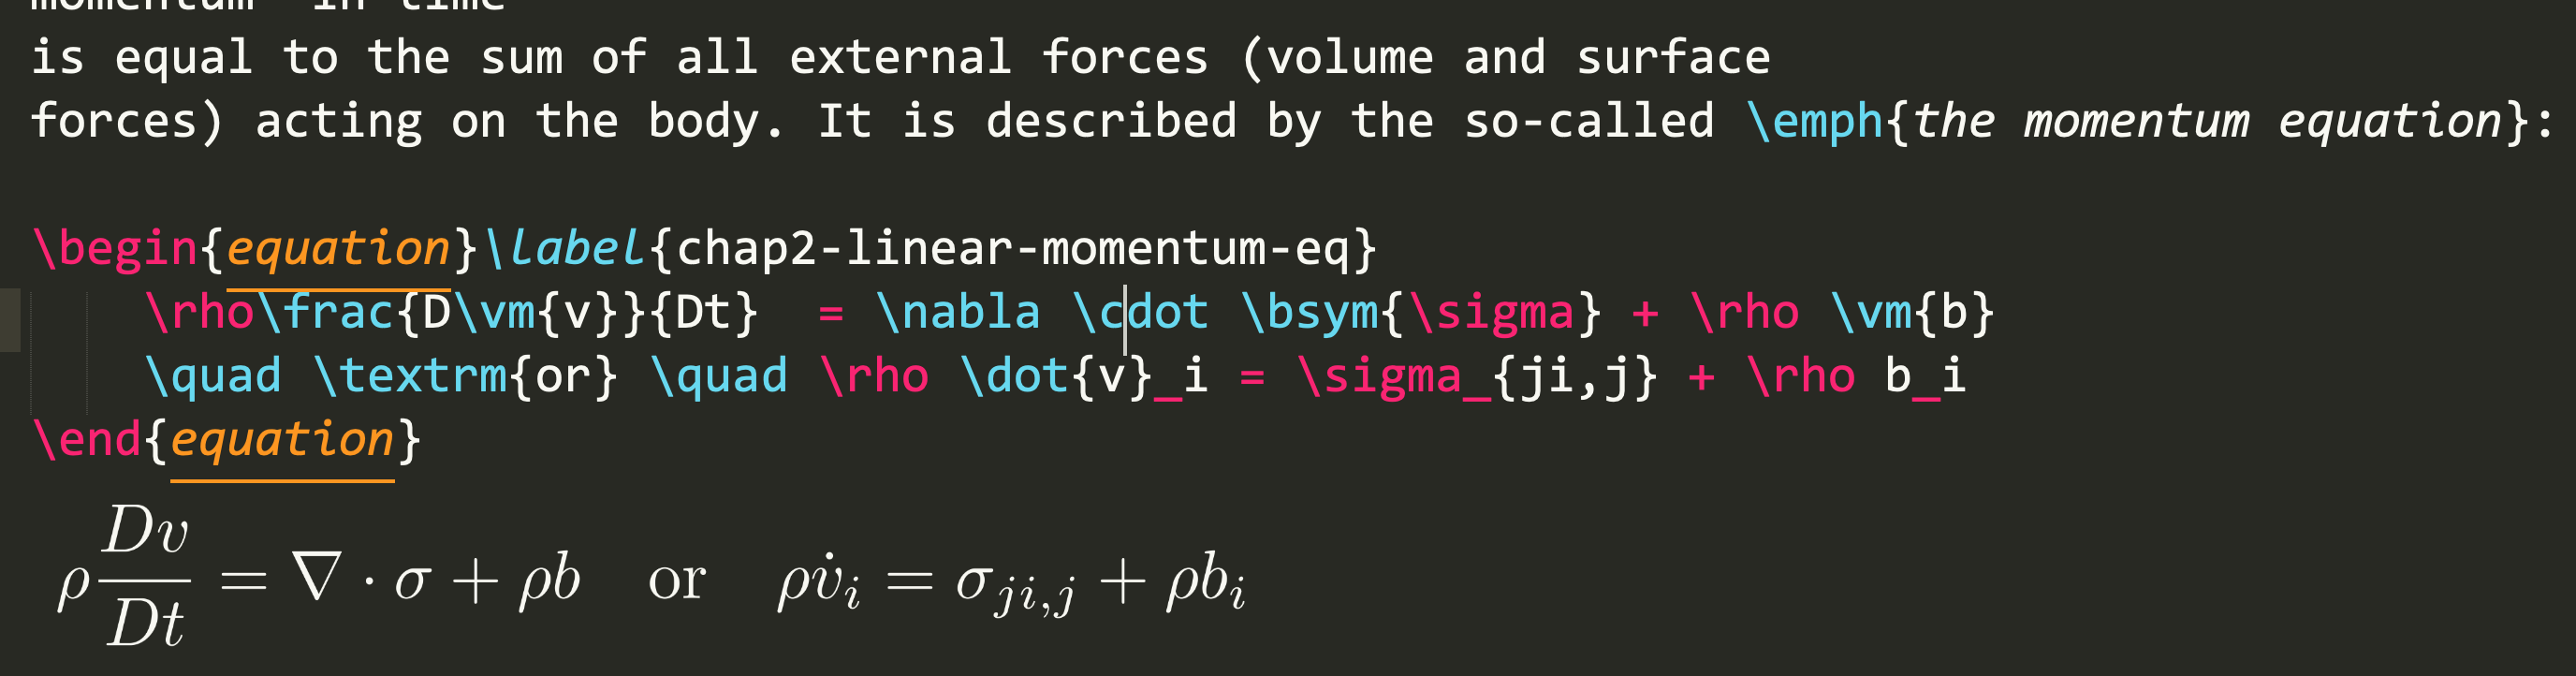
\includegraphics[width=0.65\textwidth]{sublime-text}
   \caption{\texttt{Sublime Text} can render equations in real time.}
\label{fig:sublime-text}
\end{figure}
\end{rmk}

\begin{rmk}\label{rm:a}
There are many alternatives to \texttt{matplotlib} such as \texttt{gnuplot} and \texttt{Matlab}. We used  \texttt{Matlab} and recently switched to \texttt{Python}. There are many reasons that influenced this, two of which are noteworthy. First, it is fun and beneficial to the brain to learn something new. Second, \texttt{Python} is now everywhere: it is used as a scripting language for many finite element packages (e.g. \texttt{Abaqus}) and scientific visualization programs (\texttt{Paraview} and \texttt{Ovito} for example).
\end{rmk}


The tools described in this section help you to write papers effectively, only when you have an idea how a paper should look like. The next section is devoted to just that. 

%%%%%%%%%%%%%%%%%%%%%%%%%%%%%%%
\section{Writing tips}\label{sec:writing-tips}

This section presents  writing tips. We start with a presentation of general guidelines in \cref{sec:guidelines}. Then we  discuss the paper structure in \cref{structure};  all major components of a paper are treated: title, abstract, introduction, results, conclusions, appendices, and references. Next, we discuss equations in
\cref{sec:equation} and figures in \cref{sec:citing-figs}. How to construct sentences and paragraphs is outlined in \cref{sec:sentences,sec:paragraph}, respectively.
Some common mistakes and a few tips to make your paper less verbose or wordy are given next in 
\cref{sec:mistakes}.  Finally, \cref{sec:writing-process} -- the most significant contribution of the paper -- outlines an iterative writing process in which writing is intertwined with other research activities. Recently, we realized that this technique has been, not surprisingly, adopted by other researchers, \eg \cite{Jones}.

%--------------------------------------
\subsection{General guidelines}\label{sec:guidelines}

The following general guidelines for a high quality scientific paper are nothing new but they are worth being repeated:

\begin{enumerate}
\item The purpose of a paper is to inform not to impress;
\item The writers should aim for clarity and readability and  reproducibility;
\item Contributions must be clearly stated;
\item Every unit of discourse (a sentence, a section, an article \etc), no matter the size conveys only a single idea or message \citep{gopen1990science,McCarthy}\footnote{Watch also the interesting talk of Judy Swan at \url{https://www.youtube.com/watch?v=1pzjxYCwb08}.};
\item Avoid jargon and abbreviations;%  Writing a paper is not a race for complexity. You should make it as simple as possible for a neophyte reader to understand;
\item Figures should be of high quality (\eg at least the font is legible);
\item Minimize chances for reviewers to raise issues.
\end{enumerate}

The main contributions of your paper must be clearly stated after a brief review of the literature: in which way your work differs from the existing literature. Be precise, as this is where the reviewers will try to find problems with your work. Their goal is to identify whether your work is novel or not. If it is not immediately clear from the Abstract and Introduction you risk being unconvincing. 



Avoid jargon which are the specialized vocabulary of any profession, trade, science.  Writing a paper is not a race for complexity. You should make it as simple as possible for a neophyte reader to understand.
Our advice is try to avoid jargon in the abstract and introduction as much as possible so that your paper is more accessible to a wide range of audience. In case that a jargon is needed, provide a definition for it the first time it appears in the paper, and also include clarifications for any poorly formed jargon.

Consider the following sentence appearing in an abstract:

 \begin{quote}
  \textit{There are different formulations  to model the tension/compression asymmetry of fracture.}
 \end{quote}
The jargon 'tension/compression asymmetry' might not be clear to some audiences. A better version of the above is:

 \begin{quote}
    \textit{There are different formulations  to model the tension/compression asymmetry of 
    fracture – fracture does not occur in domains under compression.}
 \end{quote}


Reproducibility is a big issue in scientific research nowadays. Reproducibility requires that findings can be verified independently.
However, we just confine ourselves here to the situation where a published simulation result is genuinely correct but impossible to reproduce by people other than the authors. The world would be a better place if all authors are more thoughtful when reporting their results: all information needed to make that particular simulation work should be provided. Particularly, nontrivial parameters.


You can save time for both you -- the authors -- and the reviewers by not making them guess. For example, if you do not do large deformation simulations, make it clear and justify that choice. If you have used a particular value for one numerical parameter, explain your choice. The bottom line is: \textit{Explain everything}; if something is obvious to you does not mean that it is obvious to your reader. If reviewers have to guess your choices, they will comment on that. This increases the chances for your paper to be rejected, or needing corrections.




%%%%%%%%%%%%%%%%%%%%%%%%%%%%%%%
\subsection{How to structure your paper}\label{structure}

Typically a paper in the field of  computational engineering and sciences consists of the following parts:

\begin{itemize}
    \item Title
    \item Abstract
    \item Introduction
    \item Methods
    \item Results
    \item Conclusions
    \item Acknowledgments
    \item Appendices
    \item References
\end{itemize}
 In this section we discuss some suggestions on how to write  these parts. We start with titles in \cref{sec:title}, which is followed by \cref{sec:abstract} on the abstract part. Then we present a way to organize long sections by having a global paragraph before going into its subsection (\cref{sec:global-para}). Next, we discuss how to write a compelling introduction section (\cref{sec:introduction-part}). After that, we discuss the results section (\cref{sec:result}) and the conclusion section(\cref{sec:conclusion-part}).  Appendices and footnotes are discussed in \cref{sec:appendix-footnotes} and references in \cref{sec:references}.

An excellent article on how to structure a scientific paper can be found at \url{https://www.nature.com/scitable/topicpage/scientific-papers-13815490/}. There are certainly overlaps between it and our discussion. 



\subsubsection{Title}\label{sec:title}

Why should you pay more attention to the title of your paper? This is because
\begin{itemize}
\item the title  is the part of a paper that is read the most;
\item it is usually read first; and thus a good title gives a good first impression;
\item papers with short titles  got more citations \citep{paiva2012articles};
\item using a question mark in a paper’s title reduces the citations;
\item using a colon tended to improve the citations.
\end{itemize}

What a good title look like then? It should

\begin{itemize}
\item indicate accurately the subject/scope of the study;
\item reveal the significance of the paper;
\item contain no abbreviations;
\item exclude phrases such as "study of," "analysis of" or similar constructions.
\end{itemize}

The following title 
\begin{quote}
  \textit{An efficient and robust staggered algorithm applied to the quasi-static description 
  of brittle fracture by a phase-field approach}
 \end{quote}
can be modified to make it better
\begin{quote}
  \textit{An efficient and robust staggered solver for a phase-field model of  quasi-static 
  brittle fracture}
\end{quote}
\subsubsection{Abstract}\label{sec:abstract}

The abstract of a paper is the most important section of your paper. This is so because it is the second section that is read by journal editors (they read your cover letter first). Furthermore, once your paper has been published, its abstract is the first section that is clearly examined by readers. And in many cases, it is the only section of the manuscript that will be ever read. Sadly, many authors write the abstract in a great rush, almost as an afterthought (probably too eager to let the paper go?).

The abstract should be a concise standalone summary of your paper. It must include the background, gaps, methodology and results. In other words, it answers these questions: Why did you do the study? What did you do?  What did you find? What did you conclude? \cref{fig:abstract} presents an example of a good abstract. We label it a good abstract because it answers the above questions and it does not contain abbreviations.

\begin{figure}[h!]
\centering
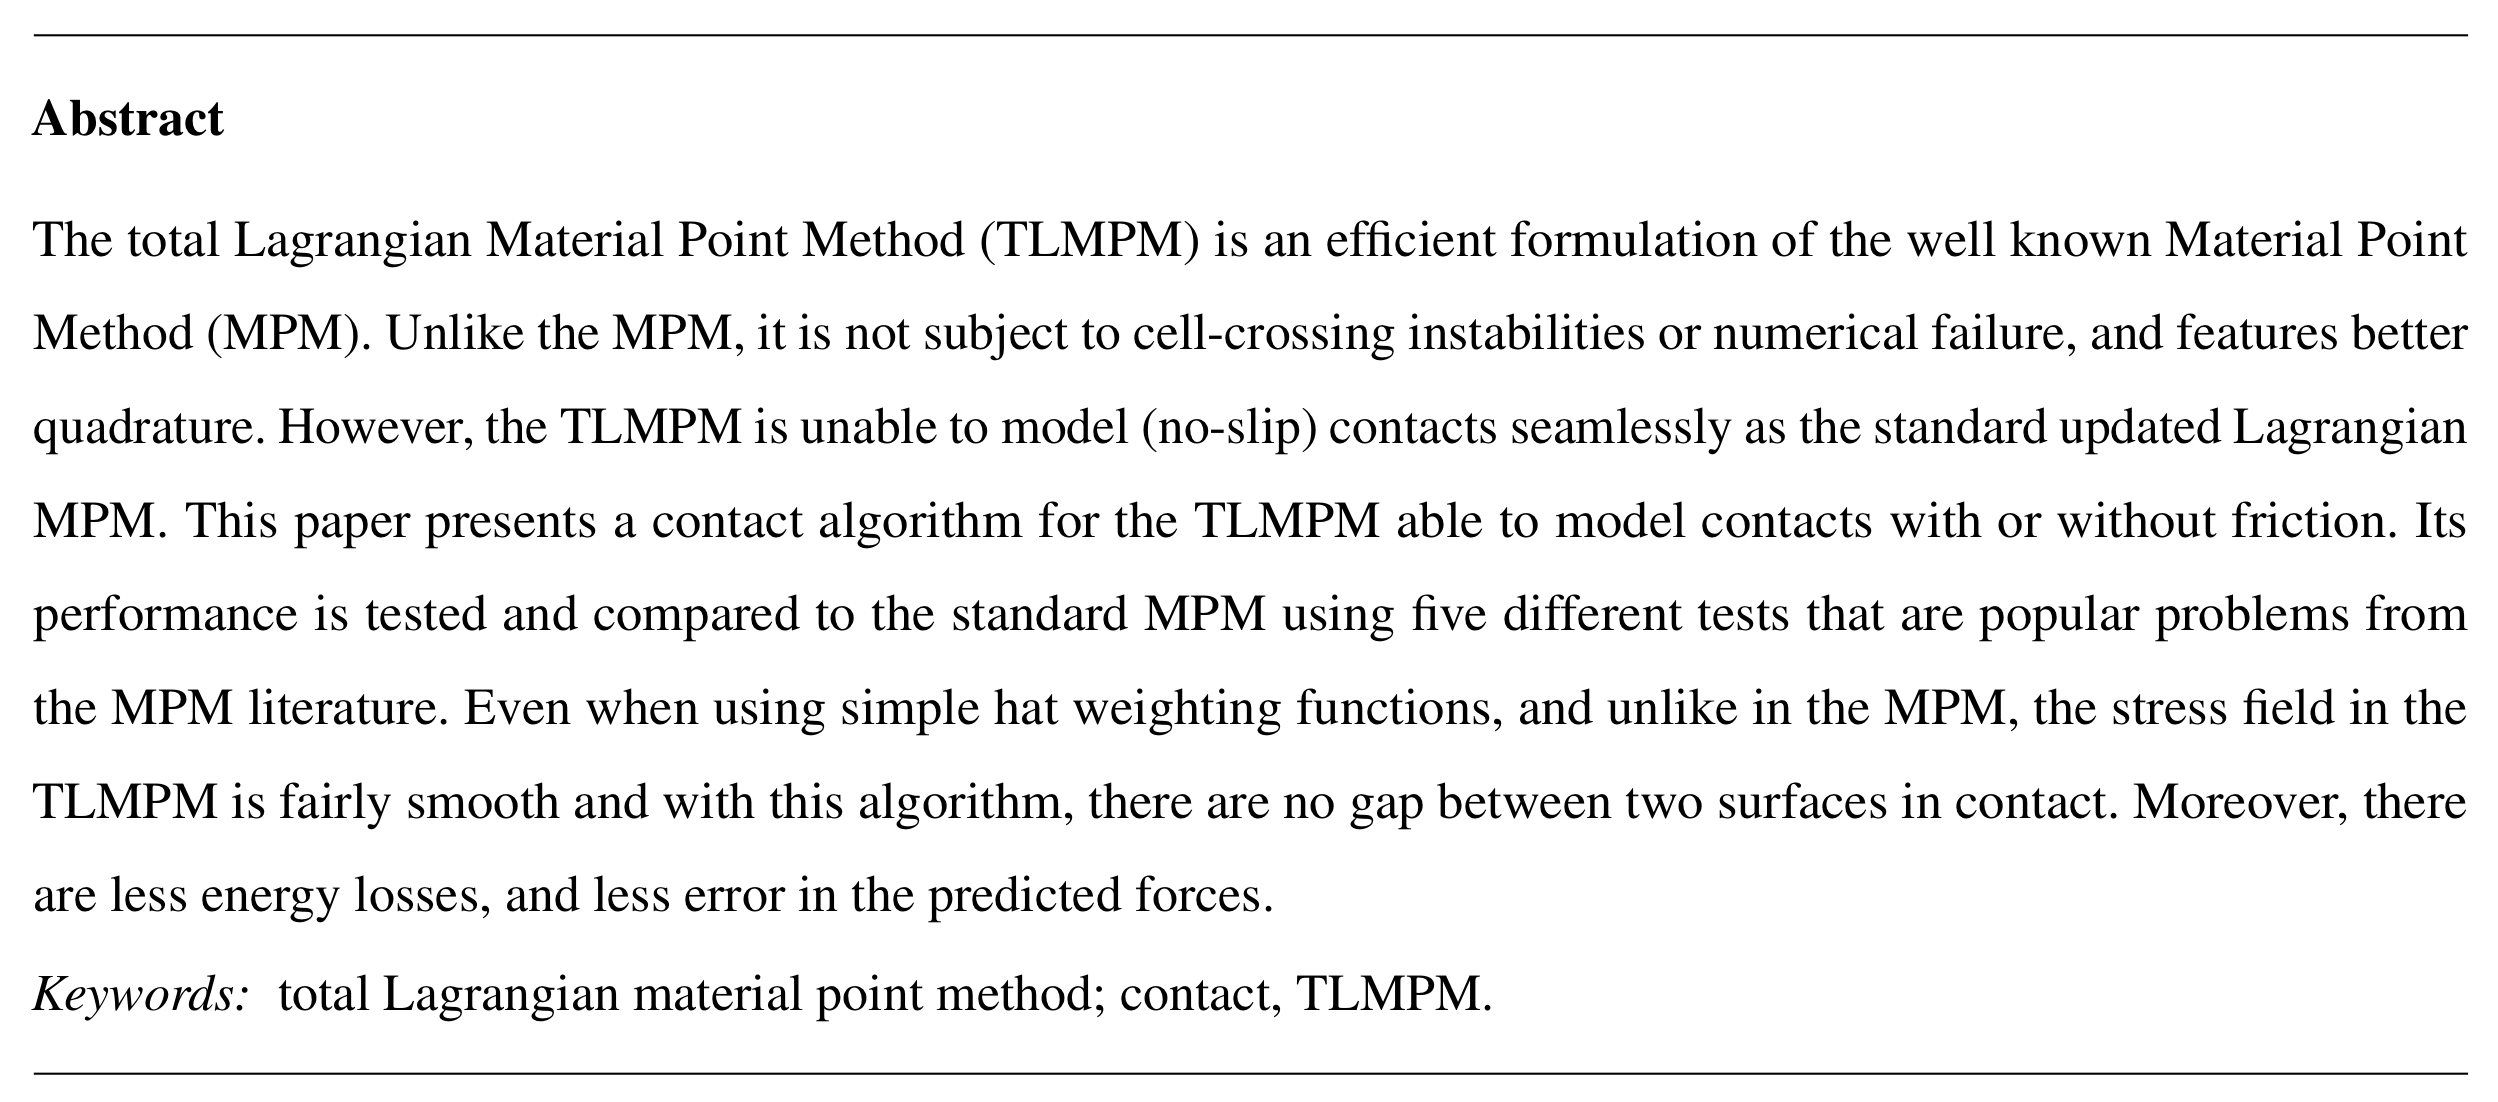
\includegraphics[width=0.86\textwidth]{abstract}
\caption{Example of a good abstract, taken from \cite{Ambati:CMAME2016a}.}
\label{fig:abstract}
\end{figure}


\subsubsection{Global paragraph for long sections}\label{sec:global-para}

For paragraphs that are quite complex it is a good idea to write a global paragraph (or mini-introduction) between the heading of a section and the heading of its first subsection. The idea is  to prepare your readers for the structure ahead at all levels; not doing so might make your reader lost. See \cref{fig:section} for an example. 


\begin{figure}[!h]
  \centering
  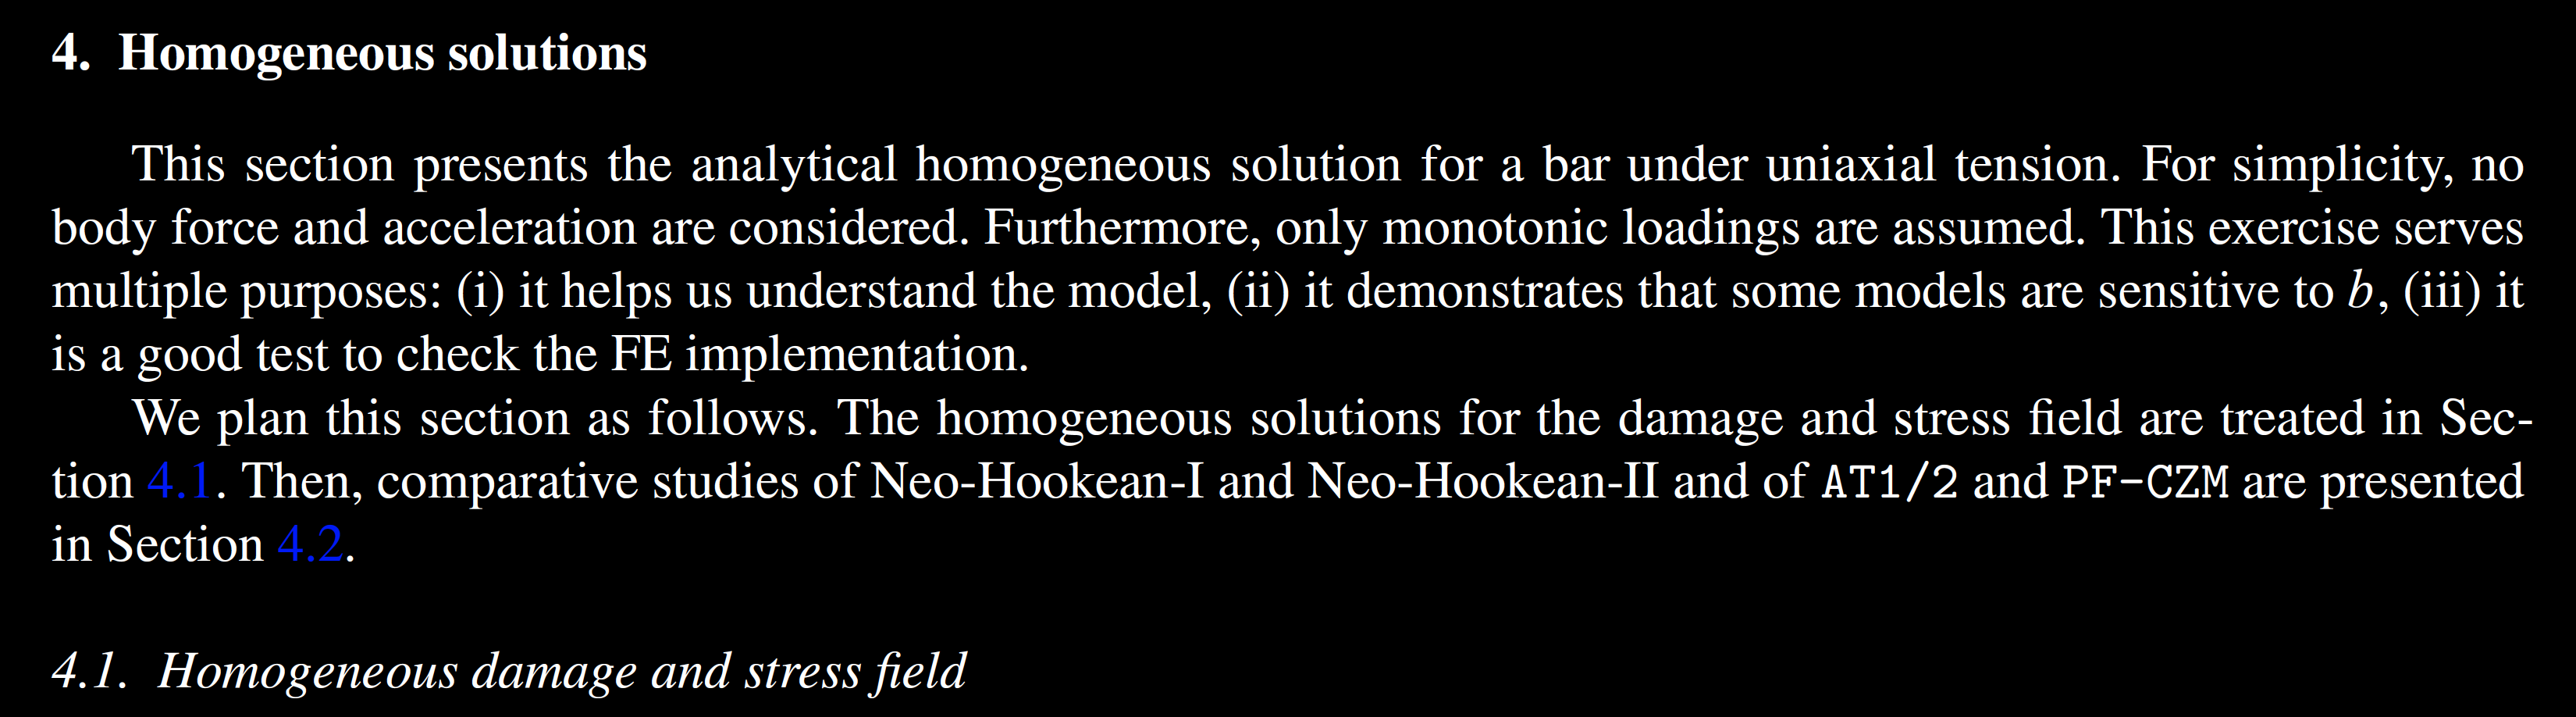
\includegraphics[width=0.9\textwidth]{section}
  \caption{A complex section should have a global paragraph between the heading of a section and the heading of its first subsection.}
  \label{fig:section}
\end{figure}


Papers on the field of computational engineering and sciences always have a section, typically named `Numerical Examples' where some tests are presented to demonstrate the performance of the model/theory presented. While these examples are most often presented in order of increasing complexity, we can do a better job in presenting them. For example, a global paragraph stating why these examples were chosen, which open source (if it is the case) code was used, etc. We first saw this technique probably in \cite{huang2003modeling}. Furthermore, a table with all parameters used for all simulations would be helpful, see \eg \cref{table:params}, as it is harder to get them if they are embedded in the text.

\subsubsection{Introduction section}\label{sec:introduction-part}

Everyone would agree that the introductory section of a paper should contain the following items, in order:

\begin{enumerate}
\item What the problem that the paper is solving;
\item Demonstration the importance of that problem;
\item What are the current approaches to solving this problem and what is wrong about them;
\item What are the contributions of the paper; 
\item Planning  the readers for reading the subsequent sections.
\end{enumerate}

It is not an easy task to write an introductory section that (i) includes all the above items, (ii) covers all relevant works, (iii) is easy to follow and (iv) is short.

What we commonly see in the literature is introductory sections of about 2 to 3 pages, full of just plain text with lots of jargons. There are two problems with this type of writing. First, only the authors and a dozens of experts can understand what is going on. Second, the paper loses many readers. We have realized that using some formula, figures, tables in the introduction section significantly improves the readability.
See \cref{algo-static-FEM} for an example, taken from \cite{Mandal:EFM2019}.

%---------------------------------------------------------------------------------------
\begin{MyBox}[label={algo-static-FEM}]
{Equations and tables can improve the introduction section.}
According to second-order PFMs for quasi-static fracture of solids under the infinitesimal strain regime, the displacement field $\bfu$ and damage field $d$ are minimizers of the following total energy functional of the solid 
\begin{equation*}
  \mathscr{E} (\bfu, d) 
    = \int_{\varOmega_{0}} \left[\omega(d)\psi_{0}^+(\bfepsilon (\bfu)) + \psi_{0}^-(\bfepsilon (\bfu)) \right]\td V
    + \int_{\varOmega_{0}}  \frac{G_\text{f}}{c_\alpha} \left[ \frac{1}{b} \alpha(d)
    + b \left( \nabla d \cdot \nabla d \right) \right] \td V
    - \mathscr{P} (\bfu)
\label{eq:3}
\end{equation*}
where the first integral is the stored strain energy, the second one denotes the fracture energy \`a la Griffith. The positive and negative parts of the strain energy density are denoted by $\psi_{0}^+(\bfepsilon (\bfu))$ and $\psi_{0}^-(\bfepsilon (\bfu))$, respectively.\\

 \begin{tabularx}{\textwidth}{lllllll}
   \toprule
 model & $\alpha(d)$ &  $\omega(d)$    & fracture type & length-scale & sup.  & Parameters\\
   \midrule     
  \texttt{AT2} & $d^2$  & $(1 - d)^{2}$  & brittle  & $b=(27/256) l_{\text{ch}}$ & $\infty$ & $E_0,\nu_0,G_\text{f},b$ \\
  \texttt{AT1} & $d$    & $(1 - d)^{2}$ &  brittle  & $b=(3/8) l_{\text{ch}}$ & $4b$  & $E_0,\nu_0,G_\text{f},b$\\
  \texttt{PF-CZM} & $2d-d^2$ & $\dfrac{(1 - d)^p}{(1 - d)^p + Q(d)}$ &  brittle/cohesive  & numerical param. & $\pi b$  & $E_0,\nu_0,G_\text{f},f_t$\\
   \bottomrule
 \end{tabularx}%
\end{MyBox}

One way to visually demonstrate the contributions of your paper is to use a table in which a comparison with previous models is given. We borrowed this idea from the computer graphics community, see e.g. \cite{Stomakhin:TG2013a}. We have adopted this idea in \cite{Vaucorbeil:AAM2019} where we have provided a table (\cref{tab:summary}) where we compared different variants of the material point method (MPM).

%%%%%%%%%%%%%%%%%%%%%%%%%%%%%%%%%%%%%%%%%%%%%%%%
\vspace*{3mm}
\begin{table*}[h!]
\centering
 \caption{Overall characteristics of common MPM variants. The smileys and frownies are typeset using the package \texttt{wasysym}. }  
  \setlength\fboxsep{0pt}
\vskip-\topsep%
\smallskip%
%\renewcommand\arraystretch{1.3}
\colorbox{darkgray}{%
 \begin{tabularx}{0.99\textwidth}{lllllll}
   \toprule
 MPM variant & Efficiency & Quad. error & Cell crossing  & Num. fracture & Grid type & Contacts \\
   \midrule     
  MPM   & \smiley{} \smiley{}  \smiley{}  & \frownie{} \frownie{} \frownie{} & yes & yes & Cartesian/unstructured & \smiley{} \\
  GIMP  & \smiley{} \smiley{}  & \frownie{} \frownie{}   & no & yes  & Cartesian & \smiley{}  \\
  CPDI  & \smiley{} \smiley{}  & \frownie{}   & no  & no  & Cartesian&  \smiley{}  \\
  TLMPM & \smiley{} \smiley{} \smiley{} \smiley{}  & \frownie{}    & no & no  & Cartesian/unstructured&  \frownie{}   \\
  iMPM  & \smiley{}  & \frownie{}   & no & n/a & n/a & n/a \\
   \bottomrule
 \end{tabularx}%
}
 \label{tab:summary}
\end{table*}

Another way to intrigue readers is to summarize all the impressive simulations that the model presented in your paper can do in a figure (see \cref{fig:all-results}). In this way, you increase the chance that your paper gets read to the end.

\begin{figure}[!h]
  \centering
  \includegraphics[width=0.5\textwidth]{mpm-all-results}
  \caption{A figure with all good results that the model in your paper can deliver can help to intrigue readers so that they will read your paper to the end. Taken from \cite{Vaucorbeil:AAM2019}.}
  \label{fig:all-results}
\end{figure}

\subsubsection{Results section}\label{sec:result}

In many fields a paper contains one section discussing the results and one section ``Discussions'' to elaborate on the results. However, in the field of computational mechanics, most often these two are combined into one section named ``Numerical examples'' or the likes.

As we have discussed in \cref{sec:global-para} for long and complex section we need to have a global paragraph planning the reader. For the Results section, this global paragraph should explain: (1) what examples are considered and for what purposes, (2) which codes are used and (3) what not considered and reason of doing so. If all these details are given it is easier for the reviewers and the researchers transitioning to a new field to know what is going on. \cref{fig:examples} presents such a global paragraph.

\begin{figure}[h!]
\centering
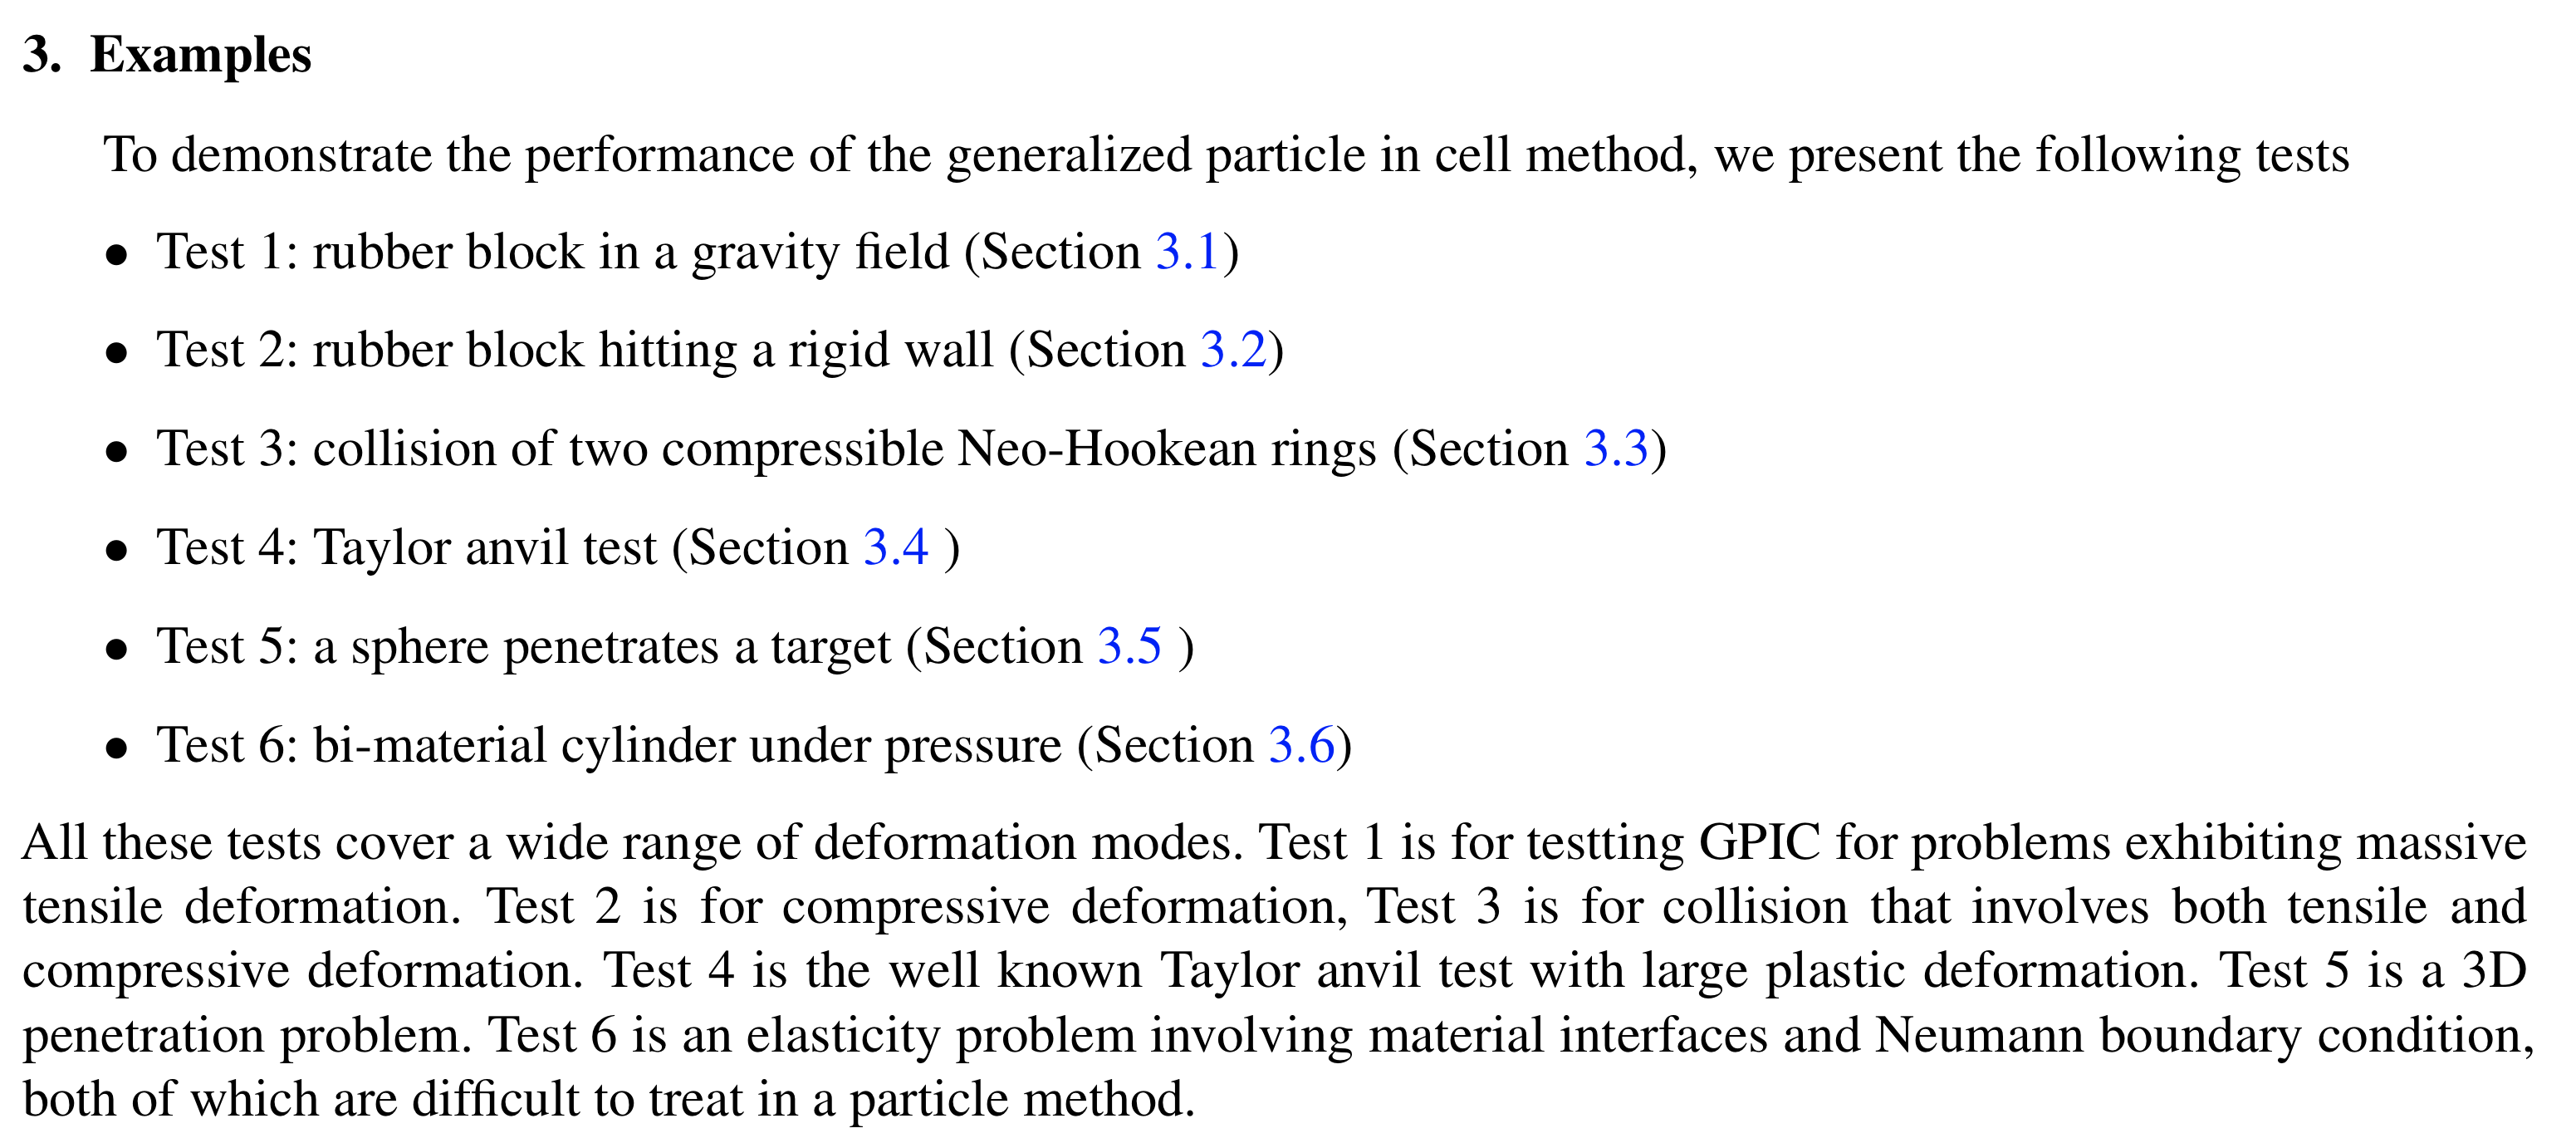
\includegraphics[width=0.87\textwidth]{examples}
\caption{A global paragraph planning the reader for the Results section.}
\label{fig:examples}
\end{figure}

For each example, before presenting the results, we should also help the reader by stating what is the question that we want to find answer with it, and what qualitative and quantitative measures are used for that purpose. For example, for example 1, we can write:

\begin{quote}
  \textit{
  The aim of this example is to verify if the proposed method provides mesh convergent results. To this end, we consider four finite element meshes of increasing number of elements, and for each mesh we monitor the load-displacement measured at point $P$ (see Fig.1). The method is said to be mesh convergence if the load-displacement plots converge for the used meshes.
  }
\end{quote}

\subsubsection{Conclusion section}\label{sec:conclusion-part}

There are two misunderstandings about the Conclusion section. First, the Conclusion section is usually made long under the false belief that a longer Conclusion will seem more impressive. Second, it is most often just a replication of the Abstract and/or part of the Introduction in a present perfect tense. If the reader has to read your Conclusion to know what your paper is all about, then your Abstract and Introduction were not well written.

Some papers with well written sections even do not have a conclusion section. We are not a fan of that and believe having a conclusion is a good thing. Following the Nature paper introduced at the beginning of this section, a well written conclusion section should include the following items:

\begin{itemize}
\item A brief summary (one or two sentences) of what the paper is about;
\item A summary of the key findings of the paper;
\item A list of potential improvements.
\end{itemize}
The key findings can be presented using bullet points. And as far as bullet points are concerned, we have to mention parallel structure. Parallel structure means that coordinate parts of a sentence, such as items in a series or list, have the same grammatical form. 

For example, in a draft version, one student of ours wrote (in the introduction section): We present the following concrete contributions:
\begin{itemize}
	\item A unified fourth order phase field fracture framework for brittle and quasi-brittle solids which can be considered as an extension of the unified PFM of Wu (2017);
	\item A semi-analytical (analytical-numerical) approach for PF-CZM;
\item A almost length scale insensitive fourth order PFM;
\item The first fourth order PFM for cohesive fracture;
\item The PF-CZM is applied to study the phenomena of crack kinking in anisotropic brittle fracture
\end{itemize}
We do not need to be a native English to recognize that the above list is wrong. Just by reading it out loud we can see that the first three bullet points are ok, but there is something wrong with the fourth and fifth bullets.

Using parallel structure, the above list must be written as follows: We present the following concrete contributions:
\begin{itemize}
	\item A unified fourth order phase field fracture framework for brittle and quasi-brittle fracture;
\item A semi-analytical approach for the fourth order PF-CZM;
\item A comparison of the fourth order PF-CZM against the second order PF-CZM;
\item A study of the phenomena of crack kinking and saw-tooth cracking in strongly anisotropic brittle fracture.
\end{itemize}

Parallel structures can be used in sentences and in paragraphs. 

\subsubsection{Appendix and footnotes}\label{sec:appendix-footnotes}

It is appropriate to include appendices when
the incorporation of material in the body of the paper would make it poorly structured or it would be too long and detailed and to ensure inclusion of supporting material that would otherwise clutter or break up the narrative flow of the paper.
As discussed later in \cref{sec:equation}, it is better to move some equations to an appendix.

There are opposite ideas about footnotes. Some authors use them scarcely and some use them extensively. The argument of the former is that footnotes \textit{break the flow of thoughts and send your eyes darting back and forth while your hands are turning pages or clicking on links} according to Pulitzer prizewinner novelist Cormac McCarthy \citep{McCarthy}. The argument of the latter is probably to reduce the paper's length. But, we find one wrong thing about footnotes: too lengthy footnotes. Some papers contain footnotes that are half a page long and with a smaller font than the main text. These are not readable.

We use footnotes sparingly and they are most often short. If you find a long footnote, consider using a remark as we have done in \cref{rm:a}.

\subsubsection{References}\label{sec:references}

You should pick one reference style and stick to it so that the references are consistent. Regarding how relevant work should be cited, below are some suggestions:

\begin{itemize}
\item Cite originals not derivatives;
\item Avoid citing a list of two many papers \eg `See [1-20] for some relevant work'. This helps neither the readers to find anything, nor the authors of [1-20] to get credit;
\item If a author-year reference format is used \eg 'Walker (1996) studied ...', all references in a single citation should be ordered in chronological order. For instance, `To help ease the writing process, books and articles giving advice on how to write scientific papers have been written \citep{day1998write,ashby2000write,plaxco2010art}.'
\end{itemize}

\subsection{Notations and equations}\label{sec:equation}

Avoid overly complex notations, see \cref{tab:complex-notation} for some examples. Try to introduce a nomenclature in the paper, to ease things for the reviewers and readers.  Sometimes, a table such as \cref{tab:notations} does a good job to introduce main notations. 

%%%%%%%%%%%%%%%%%%%%%%%%%%%%%%%%%%%%%%%%%%%%%%%%%%
\begin{table*}[h!]
   \centering
\caption{Avoid overly complex notations.}
     \setlength\fboxsep{0pt}
\vskip-\topsep%
\smallskip%
%\renewcommand\arraystretch{1.3}
\colorbox{darkgray}{%
   \begin{tabularx}{0.3\textwidth}{ll}
   \toprule
   Don't & Do  \\
  \midrule
   $\varkappa$ & $\kappa$  \\
   $\hbar$ & $\bar{h}$  \\
   $\underline{\underline{A}}$ & $\boldsymbol{A}$ or $A_{ij}$\\
  \bottomrule
 \end{tabularx}%
 }
 \label{tab:complex-notation}
\end{table*}

%%%%%%%%%%%%%%%%%%%%%%%%%%%%%%%%%%%%%%%%%%%%%%%%%%

\begin{table*}[h!]
\caption{Major notations can be put in a table.}
   \centering
     \setlength\fboxsep{0pt}
\vskip-\topsep%
\smallskip%
%\renewcommand\arraystretch{1.3}
\colorbox{darkgray}{%
   \begin{tabularx}{0.6\textwidth}{llX}
   \toprule
   Variable & Type  & Meaning\\
  \midrule
  $\mathbf{x}_p$ & Vector & Particle position (time-dependent)\\
  $\mathbf{X}_p$ & Vector & Particle initial position\\
  $m_p$ & Scalar & Particle mass\\
  $V_p$ & Scalar & Particle volume\\
  $\rho_p$ & Scalar & Particle density\\
  $T_p$ & Scalar & Particle temperature\\
  $\mathbf{P}_p$ & Tensor/Matrix & Particle 1$^\text{st}$ Piola-Kirchoff stress\\
  \bottomrule
 \end{tabularx}%
 }
 \label{tab:notations}
\end{table*}
%%%%%%%%%%%%%%%%%%%%%%%%%%%%%%%%%%%%%%%%%%%%%%%%%%

Ideally, the impact of a scientific work should be determined by its scientific merit, rather than by presentational style. Unfortunately, \cite{Fawcett11735,Higginson_2016} showed that scientifically strong papers may have reduced impact if not presented in an accessible manner. 
The density of equations in an article on ecology and evolutionary biology has a significant negative impact on citation rates, with papers receiving 28\% fewer citations overall for each additional equation per page in the main text \citep{Fawcett11735}. For papers in physics, the number is 6\% fewer citations for each additional equation per page \citep{Higginson_2016}.

The lesson to learn from the above relation between the density of equations in a paper and its impact is to write less equations in the body of the paper. This can be achieved by removing unnecessary equations. If needed, some equations can be put in appendices.

A paper in the field of computational sciences certainly contains some mathematical equations and/or expressions. To demonstrate how equations are written, we use the following one (taken from one of our papers)

\begin{equation}
  \mathscr{E} (\bfu, d) 
    = \int_{\varOmega_{0}} \left[\omega(d)\psi_{0}^+(\bfepsilon (\bfu)) + \psi_{0}^-(\bfepsilon (\bfu)) \right]\td V
    + \int_{\varOmega_{0}}  \frac{G_\text{f}}{c_\alpha} \left[ \frac{1}{b} \alpha(d)
    + b \left( \nabla d \cdot \nabla d \right) \right] \td V
    - \mathscr{P} (\bfu)   
\label{eq:energy-functional}
\end{equation}
where the first term is the strain energy, the second term is the surface energy and the third term the external energy. Collectively, they define the energy of the mechanical system $\mathscr{E} (\bfu, d)$\footnote{Any mathematical symbols appearing in the text must be typeset using a math font. In \latex this is achieved by putting the symbols in two dollar signs.}.  

Note that we have "voiced out" the above equation in "words" so that the reader will have one more way of understanding, and the equations will not look as blunt and intimidating, in particular when you have a lot of notation which does not appear in literature. Later on we refer to this equation using its number as: \textit{The energy functional in \cref{eq:energy-functional} is minimized to obtain ...}

We do not want to discuss about punctuation in equations as this problem is still a debate. Do whatever you feel comfortable with. But the editor can ask you to add punctuation in your equations!



\subsection{Figures}\label{sec:citing-figs}

Figures  are  an important element of reporting the findings of your research. The reader usually starts by reading the abstract, conclusion and figures. If the figures are self-contained and convincing, it is likely that the reviewers will accept the paper without asking a large number of questions. If they have to read the whole text to understand the worth of each figure, this will slow their progress and could make them impatient, hence decrease the chance of giving recommendation for your paper. 

A high quality figure is worth a thousand words. By a high quality figure we meant the one that has a legible font size, a high resolution, is color-blindness aware, of which all the axes are clearly defined, those sorts of things. Later on we will discuss how to prepare such figures (\cref{sec:figs}). We emphasize the importance of high quality figures because we have seen so many figures which are, without better words, of very low quality.

Tables and figures, although important components of any research papers, are just that—components; you can publish a paper without them but you cannot publish tables or figures without a paper. Thus a figure (or table) exists to support the text. So the first rule is: make sure that every table and figure is mentioned in the text. Even though there are some \LaTeX\ packages (\eg \texttt{Refcheck}) that help to find out unused figures and tables, our practice is when we insert a figure in our document, we cite it immediately. And the second rule is: remove any figure if it does not support your discussion. The third rule is good figure captions. Pay attention to the figure captions. Ideally, the reader should be able to ascertain the entire story just by reading the figure captions \ie without going back and forth between the figure and the text sections. And the final is how figures/tables are referred to in the text.

One usually does not pay enough attention to how figures (and tables) should be referred to in the text. That is why one usually write the following sentences

 \begin{quote}
  \textit{Fig. 10 depicts the global responses. As can be seen, the global responses are 
  insensitive to the incorporated length scale.}
 \end{quote}
The first sentence is unnecessary as it only directs the reader to the figure (Fig. 10), and thus it provides no information. We have found similar sentences in the literature (including our papers). A better version of the above is:

 \begin{quote}
  \textit{The global responses are insensitive to the incorporated length scale (Fig. 10).}
 \end{quote}
We say that this is a better version because it did not use the phrase `As can be seen'. It is clear that the use of too many such phrases should (and can be) be avoided. 
Actually we already use this style when we cite published articles and books to support an argument. We can do the same thing with figures and tables.

\subsection{Sentences}\label{sec:sentences}

We recommend the advice of the Pulitzer prizewinner Cormac McCarthy \citep{McCarthy}

\begin{quote}
Keep sentences short, simply constructed and direct. Concise, clear sentences work well for scientific explanations. Minimize clauses, compound sentences and transition words — such as ‘however’ or ‘thus’ — so that the reader can focus on the main message.
\end{quote}
Don't worry too much about grammatically perfect sentences. It is more important to be understood \citep{McCarthy}. 


\noindent\textbf{Passive vs active voice}.     Sentences can be written using either an active voice  or passive voice. The active voice focuses on the agent: "David measured the temperature." (Here, the agent--David--is the subject of the sentence). In contrast, the passive voice focuses on the object that is acted upon: "The temperature was measured by David". 

To choose between active and passive voice, consider what you are discussing and place it in the subject position. Using the above example of measurement of temperature, it is obvious that the temperature is the focus. So, we should write: "The temperature was measured." David was omitted because no matter who measured the temperature we would expect its value to be the same. And this demand for objectivity of the writing has led to an overuse of the passive voice in scientific writing. For example, we see  sentences similar to the below one all the time:

\begin{quote}
\textit{In this section, a discussion of the influence of the temperature on the deformation of ... is presented.}
\end{quote}
This sentence is not only boring but also verbose. Look at the following equivalent sentence using an active voice:

\begin{quote}
\textit{This section discusses the influence of the temperature on the deformation of ...}
\end{quote}
This sentence is shorter and easier to understand. Therefore, a systematic preference for the passive voice is by no means optimal. Use both in your papers and note that using a personal tone can help to engage a reader. 

\subsection{Paragraphs}\label{sec:paragraph}

Each paragraph conveys only a single idea or message. Do not be afraid of writing short paragraphs, even two-sentence ones. 
Use simple sentences that are linked together so that your writing is coherent. 
See \cref{version1} for a paragraph that was not well written: the second sentence is not related to the first one and 'this issue' in the third sentence was not clear. A better version is shown in \cref{version2} where the writing is more coherent: sentences start with familiar (old) information and end with unfamiliar (new) information. We prefer the new, important information at the end, because its job is to intrigue the reader. Another example is, from S.P. Jones (yes, the same Jones who has written the interesting paper on how to write great papers \citep{Jones})


\begin{quote}
\textit{Security proofs} of cryptographic protocols are crucial for the security of everyday electronic communication. However, \textit{these proofs} tend to be complex and difficult to get right. To make it easier to manage \textit{such proofs}, Jones et al. have proposed a new design principle, called the \textit{game-playing technique}. 
\textit{This technique} follows a code-based approach where the security properties are formulated in therms of probabilistic programs, called games.
\end{quote} 
We refer to the old article of \cite{gopen1990science} for more examples of writing readable paragraphs.

Try to revise your writing to keep only the words/figures/tables that are necessary: The main message of \textit{The Elements of Style} is to omit unnecessary words \citep{white1972elements}. For example, using `because' is more advisable than the wordy `due to the fact that' (see \cref{tab:mistakes} for a list of unnecessary words/phrases).\\

\begin{MyBox}[width=0.48\textwidth,nobeforeafter,label={version1}]
{Version 1.}
{\tcbfontsize{0.8}
In the phase-field modeling of fracture in brittle and quasi-brittle solids, it is crucial to represent the \textbf{asymmetric tensile/compressive material behavior}. \textbf{Existing phase-field models generally adopt either an intuitive split of the free energy density without capturing the crack boundary conditions properly or an ad hoc hybrid formulation at the loss of variational consistency}. \textbf{To address this issue}, this work presents a variationally consistent phase-field anisotropic damage model.}
\end{MyBox}\hfill
\begin{MyBox}[width=0.48\textwidth,nobeforeafter,label={version2}]
{Version 2.}
{\tcbfontsize{0.8}
In the phase-field modeling of fracture in brittle and quasi-brittle solids, it is crucial to represent the \textbf{asymmetric tensile/compressive material behavior}. \textbf{To capture this asymmetric behavior}, previous phase-field models  generally adopt either and intuitive split of the free energy density without capturing the crack boundary conditions properly ... This work presents a phase-field anisotropic model that is able to capture \textbf{the asymmetric behavior}, \textbf{variationally consistent} and satisfy \textbf{crack boundary conditions}.}
\end{MyBox}



% 
%--------------------------------------
\subsection{Some common mistakes}\label{sec:mistakes}


Some common mistakes are given in \cref{tab:mistakes}. You could have avoided these mistakes by carefully studying the writing of your favorite author (who ever she/he is). Anyway, we collect them here in one table as a checklist.

%%%%%%%%%%%%%%%%%%%%%%%%%%%%%%%%%%%%%%%%%%%%%%%%%%
\begin{table*}[h!]
\caption{Some common mistakes. A good way to improve your writing is by reading your writing, including all of the writing out loud. Your ears can often pick out sentence fragments and grammatical errors better than your eyes. If you find yourself saying a series of fragmented sentences or feeling something unnatural, you should do some rewriting.}
   \centering
     \setlength\fboxsep{0pt}
\vskip-\topsep%
\smallskip%
%\renewcommand\arraystretch{1.3}
\colorbox{darkgray}{%
   \begin{tabularx}{\textwidth}{ll}
   \toprule
   Don't/Avoid & Do/Use  \\
  \midrule
  \textbf{The} Table/Figure 2 & Table/Figure 2 \\
  \textbf{The} Equation (2.2) & Equation (2.2) \\
  \textbf{The} Young's modulus &  Young's modulus, or the Young modulus\\
  Start a section with a table/figure/equation & Start a section with text\\
  This topic has interested researchers for a \textbf{long} time & ... for more than 20 years\\
  A \textbf{bad} result & A poor/negative result\\
  This section \textbf{serves} to explain & This section explains\\
  It is \textbf{obvious/clear} ... & \\
  \textbf{Due to the fact that} ... & Because ...\\
  \textbf{It should be noted that} there are 5 samples in this study& This study consisted of 5 ...\\
  \textbf{In order to} include ... & To include ...\\
  The difference was \textbf{found to be} significant & The difference was significant \\
  We plotted the data \textbf{by} using ... & We plotted the data using ...\\
  Utilize or usage & Use \\
  We \textbf{think/believe/feel} that the results are good & The results are good \\
  \textbf{Existing} works ... & Previous work \\
  Using adjectives such as `very', `always', `never' & \\
  Using words like `ground-breaking', `paradigm shift' & \\ 
  Using 'Above-mentioned' or 'aforementioned' & \\
  & Always spell out an acronym the first time it is used \\
  Use long titles & Use short titles  \citep{paiva2012articles}\\
   & Use a spell checker to get rid of all spell errors\\
  %Passive voice & Active voice \\
  \bottomrule
 \end{tabularx}%
 }
 \label{tab:mistakes}
\end{table*}

Most scientific papers will include numbers. Write out all numbers less than 10 (\ie seven not “7”). Write out any number at the start of a sentence. For sentences starting with long numbers, it is usually best to rearrange so that the long numbers are not at the beginning.





%--------------------------------------
\subsection{Writing process: an iterative process}\label{sec:writing-process}

The  first idea of the presented writing process is that when you have finished your last simulation, the first draft of your full paper is complete. Here, by \textit{you}, we mean the co-author of the paper who is in charge of the writing. After that, it just comes down to polishing the paper. The second idea is to not lose motivation due to set backs. That is, if the simulations are not working, don't be upset; let's write something instead. It can be as easy as filling Section \textit{Acknowledgments}. Having updated your paper will definitely make you feel good. And that is very important. The third idea is that writing is intertwined with all other activities (formulation, coding and running simulations) as illustrated in \cref{fig:writing}. 

 \begin{figure}[!ht]
      \centering
      \includegraphics{writing.pdf}
      \caption{Writing is intertwined with other activities of the project.}
      \label{fig:writing}
    \end{figure}

After a research idea has been developed, you should start writing the paper \citep{Gray:2005a}. Obviously, the paper is empty, see \cref{snippet_template} for a \LaTeX\ file for an empty paper.
For the sake of presentation, let's assume that you need to develop a formulation, implement it in a code, and carry out simulations using this code. You first work on the formulation. Then, when there is some progresses, you can write some key equations in the paper (filling Section \textit{Methodology}). Having the formulations nicely written in a PDF can help you to spot errors and to crystallize your thinking. Now that the formulation is complete, let's move to the implementation. Again, this task should be intertwined  with the writing as well (filling Section \textit{Methodology}). Most often, you start with a very simple problem to test the code (and the idea). If this example works, you become more confident about the idea, you can write something on Section \textit{Introduction} while the second simulation is under way. If this second example is important, you can write about it in Section \textit{Examples}. If you are lucky, the result of this second simulation is  good. Bingo, you can now fill  Sections \textit{Introduction} and  \textit{Abstract} while working on the third simulation.
%---------------------------------------------------------------------------
\begin{figure*}[!h]
  \begin{snippetlatex}[caption={A starting \LaTeX\ file (file with extension .tex). The paper is not formatted to any specific journal. Change the template (documentclass) accordingly for the publisher you plan to submit your paper. Introducing a table of content helps to see
  the overall structure of the paper. For brevity, packages used were skipped, see \cref{snippet_latex_packages}. \LaTeX\ keywords are highlighted in \textcolor{blue}{\textbf{bold blue font}}.  },label={snippet_template},framerule=1pt,tabsize=3]
    \documentclass[authoryear,fleqn]{article}
    \usepackage{amsmath,arxiv} % see  Listing 2 for packages 
    \makeatletter
\renewcommand\fs@ruled{\def\@fs@cfont{\bfseries}\let\@fs@capt\floatc@ruled
\def\@fs@pre{\hrule height 1.2pt depth0pt \kern2pt}%
%\def\@fs@post{\hrule height1.2pt depth0pt \kern2pt}%
\def\@fs@post{\kern2pt\hrule height 1.2pt depth0pt \kern2pt \relax}%
\def\@fs@mid{\kern2pt\hrule\kern2pt}%
\let\@fs@iftopcapt\iftrue}
\makeatother

% index generation
% see LATEX companion p 354
\newcommand{\bs}{\symbol{'134}}%print backslash
\newcommand{\Com}[1]{\texttt{\bs#1}%
\index{#1@\texttt{\bs#1}}}
\newcommand{\Prog}[1]{\texttt{#1}%
\index{#1@\texttt{#1} program }}

% shortcuts

% inner product <x,y>
\newcommand{\ipn}{\langle \cdot , \cdot \rangle}
\newcommand{\ip}[2]{\langle #1 , #2 \rangle}

% norm ||x||
\newcommand{\normn}{\left|\left| \cdot \right|\right|}
\newcommand{\norm}[1]{\left|\left|#1\right|\right|}
\newcommand{\meas}[1]{\left|#1\right|}

% McAuley brackets <x>
\newcommand{\mcauley}[1]{\langle #1 \rangle}

\newcommand{\x}{~$\times$~}
\newcommand{\fig}{Fig.~}
\newcommand{\eref}[1]{(\ref{eq:#1})}
\newcommand{\sref}[1]{\ref{section:#1}}
\newcommand{\fref}[1]{\ref{fig:#1}}
\newcommand{\tref}[1]{\ref{table:#1}}
%\newcommand{\eref}[1]{Eq.~(\ref{#1})}
%\newcommand{\erefs}[1]{Eqs.~(\ref{#1})}
%\newcommand{\fref}[1]{Fig.~\ref{#1}}
%\newcommand{\frefs}[1]{Figs.~\ref{#1}}
%\newcommand{\tref}[1]{Table~\ref{#1}}
\newcommand{\trefs}[1]{Tables~\ref{#1}}
%\newcommand{\sref}[1]{Section~\ref{#1}}
\newcommand{\srefs}[1]{Sections~\ref{#1}}
\newcommand{\crefs}[1]{Chapters~\ref{#1}}
\newcommand{\aref}[1]{Appendix~\ref{#1}}
\newcommand{\tsty}{\textstyle}
\newcommand{\dsty}{\displaystyle}
\newcommand{\D}{\displaystyle}
\newcommand{\arrow}{~$\rightarrow$~}
\newcommand{\otheta}{\overline \theta}
\newcommand{\mathG}{\mathcal{G}}

\newcommand{\mi}{_\mathrm{m}}
\newcommand{\ma}{_\mathrm{M}}

\newcommand{\Mi}{^\mathrm{m}}
\newcommand{\Ma}{^\mathrm{M}}

\newcommand{\dep}{_\mathrm{d}}
\newcommand{\ind}{_\mathrm{i}}

\newcommand{\di}{\mathrm{d}}

\newcommand{\defi}{\mathrel{\mathop:}=}

% abbreviations

\usepackage{xspace}
\newcommand{\eg}{e.g.,\xspace}
\newcommand{\EG}{e.g.,\xspace}
\newcommand{\FEG}{\textit{e.g.}\,}     % i.e.
\newcommand{\feg}{\textit{e.g.}\,}     % i.e.
\newcommand{\ie}{i.e.,\xspace}
\newcommand{\IE}{i.e.,\xspace}
\newcommand{\CF}{\textit{cf.}\,}     % i.e.
\newcommand{\cf}{\textit{cf.}\,}     % i.e.
\newcommand{\etc}{etc.\@\xspace}
\newcommand{\ETC}{etc.\@\xspace}
\newcommand{\ETAL}{et. al.\@\xspace}
\newcommand{\etal}{et. al.\@\xspace}
\newcommand{\cmatrixb}{\left\{ \begin{matrix}}
\newcommand{\cmatrixe}{\end{matrix} \right\}}

% general vector/matrix commands:

\newcommand{\tvm}[1]{\textbf{#1}}
\newcommand{\tvms}[1]{$\boldsymbol{#1}$\ }
\newcommand{\vm}[1]{\mathbf{#1}}
\newcommand{\vms}[1]{\mathbf{#1}}
\newcommand{\bsym}[1]{\boldsymbol{#1}}

% vector/matrix for space coordinates 'x' and 'y'

\newcommand{\vx}{\mathbf{x}}
\newcommand{\vy}{\mathbf{y}}
\newcommand{\ve}[1]{\mathbf{e}_{#1}}
\newcommand{\bx}{\boldsymbol{x}}
\newcommand{\vxI}{\mathbf{x}_{I}}
\newcommand{\vj}[1]{\mathbf{#1}_{j}}
\newcommand{\xI}{x_{I}}
\newcommand{\yI}{y_{I}}
\newcommand{\hvx}{\hat{\mathbf{x}}}
\newcommand{\hx}{\hat{x}}
\newcommand{\hy}{\hat{y}}

\newcommand{\trans}{^\mathrm{T}}
\newcommand{\transi}{^\mathrm{-T}}
\newcommand{\el}{_\mathrm{e}}
\newcommand{\pl}{_\mathrm{p}}

\newcommand{\inte} [1]{\int_\Omega #1 d\Omega}
\newcommand{\intE}[1]{\int_{\Omega_0} #1 d\Omega_0}
\newcommand{\intg}[1]{\int_{\Gamma} #1 d\Gamma}
\newcommand{\intG}[1]{\int_{\Gamma_0} #1 d\Gamma_0}



%\newcommand{\T}{\underline{\vm{T}}}

% Shortcuts for making slides

\newcommand{\fontone}{\bfseries\Large}
\newcommand{\fonttwo}{\bfseries\large}
\newcommand{\fontonesc}{\scshape\Large}
\newcommand{\fonttwosc}{\scshape\large}
\newcommand{\fontthree}{\bfseries}
\newcommand{\bc}{\begin{center}}
\newcommand{\ec}{\end{center}}
\newcommand{\bitem}{\begin{itemize}}
\newcommand{\eitem}{\end{itemize}}

% ************************ MATH TYPE MACROS **************************
\newcommand{\mth}[1]{\mathit{#1}}      % print standard math italics
\newcommand{\boldsym}[1]{\mbox{\boldmath${#1}$}}
\newcommand{\vct}[1]{\boldsym{#1}}     % print vector
\newcommand{\fnc}[1]{\prno{#1}}        % print function i.e. sin ...
\newcommand{\mtx}[1]{\mathbf{#1}}      % print matrix
\newcommand{\msc}[1]{\mathcal{#1}}     % print script
\newcommand{\mss}[1]{\mathsf{#1}}      % print sans sarif
\newcommand{\tns}[1]{\boldsym{#1}}     % print tensor
\newcommand{\dbl}[1]{\mathbb{#1}}      % print sets letters like |R |C, etc...
%\newcommand{\Grad}{\stackrel{\rightharpoonup}{\boldsym{\nabla}}\!\!}
                                       % print gradient operator
\newcommand{\GradL}{\!\!\stackrel{\leftharpoonup}{\boldsym{\nabla}}}
                                       % print gradient operator
\newcommand{\Grad}{\boldsym{\nabla}}
                                       % print gradient operator
\newcommand{\Div}{\Grad\cdot}          % print divergnece operator
\newcommand{\DivL}{\cdot\GradL}        % print divergnece operator

\newcommand{\ljump}{\lbrack \! \lbrack } % print left jump oerator
\newcommand{\rjump}{\rbrack \! \rbrack } % print right jump oerator
                                         % derivative
\newcommand{\jump}[1]{\ljump {#1} \rjump} % jump operator
\newcommand{\derivv}[2]{ \frac{d^2 {#1} }{d {#2}$^2$ } }
\newcommand{\deriv}[2]{ \frac{d {#1} }{d {#2} } }   % partial derivivative
\newcommand{\pderiv}[2]{ \frac{\partial {#1} }{\partial {#2} } }
\newcommand{\testspc}{\mathcal{V}}
\newcommand{\trialspc}{\mathcal{S}}

\newcommand{\volint}[1]{\int_{\Omega}\,{#1}\,dV} % integrals
\newcommand{\bndint}[2]{\int_{#1}\,{#2}\,dS}

\newcommand{\beq}{\begin{equation}}
\newcommand{\eeq}{\end{equation}}
\newcommand{\beqa}{\begin{eqnarray}}
\newcommand{\eeqa}{\end{eqnarray}}

%--My own definitions--

\newcommand{\reals}{{\mathbb R}}
\newcommand{\dof}{\emph{dof}}
\newcommand{\dofs}{\emph{dofs}}
\newcommand{\bfalfi}{\mbox{\boldmath$\alpha$\unboldmath$_i$}}
\newcommand{\bfalfj}{\mbox{\boldmath$\alpha$\unboldmath$_j$}}
\newcommand{\remark}[2]{\vspace{0.1cm}
\noindent {\bf Remark #1:}  {#2}  \vspace{0.1cm}}
\newcommand{\invisible}[1]{}
\newcommand{\bgl}[1]{\mbox{\boldmath$#1$\unboldmath}}
\newcommand{\parti}[2]{\frac{\partial #1}{\partial #2}}

% X-FEM related
\newcommand{\xfemlong}{\textit{eXtended Finite Element Method}\,}     % extend..
\newcommand{\xfem}{\textit{X-FEM}\,}     % x-fem

% ********************** VERBATIM AND IGNORE *************************
\newcommand{\bv}{\begin{verbatim}}
\newcommand{\V}{\verb}                  % EX: \V=-d{#@~}= Expr must
                                        % fit on a line

% ************************ FIGURE COMMANDS ***************************
\newcommand{\testpix}[1]{\fbox{\begin{minipage}[c]{\textwidth}
                      #1 \end{minipage} }}

%\ifpdf
% \newcommand{\putfig}[2]{\includegraphics[scale=#2]{#1.pdf}}
%\else
% \newcommand{\putfig}[2]{\includegraphics[scale=#2]{#1.eps}}
%\fi

\newcommand{\putpstex}[1]{\includegraphics{#1.pstex_t}}
% END FIGURE COMMANDS
   % shortcuts for long latex commands in 1 place
    \title{\textbf{Title of your paper}}
    \author{...}
    \begin{document}
    \maketitle
    \begin{abstract}
     % put your abstract here
    \end{abstract}
    \keywords{
      scientific writing \and \LaTeX \and scientific publication.}
    \tableofcontents            % TOC
    \section{Introduction}
    \section{Methodology}
    \section{Examples}
    \section{Conclusions}
    \section*{Acknowledgments}
    \begin{appendices}           % remove this if you do not have appendices
    \end{appendices}
    \bibliographystyle{abbrvnat} % bib style
    \bibliography{mpm}           % bib file
    \end{document}
  \end{snippetlatex}
\end{figure*}
%---------------------------------------------------------------------------



If you feel stuck at writing any parts of the paper, feel free to do something else because keeping focusing on the writing does not always help. Most often, ideas come when you are in a diffuse mode, a concept proposed in \cite{Oakley:2018a}. For example, while playing with your kids on a playground, the idea for writing a good abstract usually comes. Jotting down the idea on a phone and you're done with this part of the paper.

While working on a paper, you read the literature (we always read it anyway). If you find a good paper relevant to your work, put it in \texttt{Bibdesk} or \texttt{JabRef}, and cite it in the paper with some key sentences about it. Doing so saves you a lot of time by not re-discovering this paper in the future. Note that \texttt{Bibdesk} (or \texttt{JabRef}) can link a PDF to a paper. Therefore, we can have a library of papers on top of a \texttt{.bib} file. 

Continuing this process, by the time the final simulation has been finished, you already have a nearly complete paper. Note that you have already revised your paper many times when your simulations were running (which usually take a long time).
You just need to write the conclusions. And voila, you have a complete paper. That is why we call this writing process an effortless experience.
Before submission, there are some steps discussed in \cref{sec:submission} that need to be done.

Don't worry about the size of the paper while you are working on it. Put as many details as you feel needed. You might end up with, not a paper, but a long report (but in a format of a paper). If this is the case, keep this report (which can be used later, for instance, in your books), save it as another \LaTeX\ file and remove unnecessary parts.

Now you know what a good quality scientific paper looks like and you are ready to compile such one. The next section presents some suggestions on how to do this electronically using \LaTeX. Note that the next section is not a \LaTeX tutorial. It aims to be a starting point for your \LaTeX\ journey.

%---------------------------------------------------------------------------------------
% 


%%%%%%%%%%%%%%%%%%%%%%%%%%%%%%%
\section{\LaTeX\ tips}\label{sec:latex}

We present in this section some \LaTeX\ tips which have been collected over the years. In \cref{sec:packages}, we list the must-have packages. Then, we discuss how to prepare high quality plots in \cref{sec:figs}, tables in 
\cref{sec:tabs},  equations in \cref{sec:equation-latex}, algorithms in \cref{sec:algorithm} and source code in \cref{sec:source-code}. Modifications required for preparing two-column format papers are presented in \cref{sec:two-col}. 
To help people new to \LaTeX\ \cref{sec:latex-installation} presents its installation.

%%%%%%%%%%%%%%%%%%%%%%
\subsection{Packages}\label{sec:packages}


To improve the writing experience, once in a while we update our \LaTeX\ skills by learning the best practices and best packages. \cref{snippet_latex_packages} provides an updated list of \LaTeX\ packages being used to write our papers.
We do not plan to discuss all the packages. Instead, we want to discuss two packages: \texttt{hyperref} and \texttt{cleveref} which are useful.

By setting the option \textit{backref=page} for the package \texttt{hyperref}, there appears `Cited on page \#' at the end of all references which are back-references  to the page(s)  in which a given reference was cited.


Using standard cross-referencing in \LaTeX\ only produces the label number, a name describing the label such as figure, chapter or equation has to be added manually. The \texttt{cleveref} package overcomes this limitation by automatically producing the label name and number:

\begin{verbatim}
\cref{fig:figure1},  instead of Fig.~\ref{fig:figure1}
\cref{eq:equation1}, instead of Eq.~\ref{eq:equation1}
\end{verbatim}

%---------------------------------------------------------------------------
\begin{figure*}[!h]
  \begin{snippetlatex}[caption={Commonly used \LaTeX\ packages.},label={snippet_latex_packages},framerule=1pt,tabsize=3]
    \usepackage{amsmath,amssymb, mathtools,mathrsfs,stmaryrd,titletoc}
    \usepackage{natbib}
    \usepackage[scaled=0.92]{helvet}  % set Helvetica as the sans-serif font
    \renewcommand{\rmdefault}{ptm}    % set Times as the default text font
    \usepackage[retainorgcmds]{IEEEtrantools}
    \usepackage[usenames]{color}
    \usepackage{tabularx}    % tables
    \usepackage{booktabs}    % better tables
    \usepackage{multirow}    % multi-row tables
    \usepackage[font=small,labelfont=md]{caption,subfig} % sub-figures (see Fig. 6)
    \usepackage[most]{tcolorbox} %colored/framed text boxes with headline (see Box 1)                  
    \usepackage[bookmarks=true,colorlinks=true,linkcolor=blue,backref=page]{hyperref}
    \usepackage{float}         % make new float environment such as boxes (captioned)
    \usepackage{listings}      % insert source code \eg LaTeX and Python codes 
    \usepackage{algorithm}     % flow wrapper for algorithm
    \usepackage{algpseudocode} % second algorithm typesetting environment
    \usepackage[activate={true,nocompatibility},final,tracking=true,kerning=true,
    spacing=true,factor=1100,stretch=10,shrink=10]{microtype}%Micro-Typographic Improve.
    \usepackage{nicefrac}             % type inline fractions: \nicefrac{1}{2}
    \usepackage{numprint}             % \numprint{10000} => 10 000 not 10000
    \usepackage[title,titletoc,toc]{appendix}
    \usepackage[capitalise]{cleveref} %Basically, cleveref must be loaded last.
    \definecolor{darkgray}{rgb}{0.95,0.95,0.95} % color used in tables
    \crefname{figure}{Fig.}{Figs.}  
    \crefname{equation}{Equation}{Equations}
    \renewcommand*{\backref}[1]{}
    \renewcommand*{\backrefalt}[4]{[{%
        \ifcase #1 %
              \or Cited on page~#2%
              \else Cited on pages #2%
        \fi%
        }]}
  \end{snippetlatex}
\end{figure*}
%---------------------------------------------------------------------------



%%%%%%%%%%%%%%%%%%%%%%
\subsection{Figures}\label{sec:figs}



This section discusses how to generate high quality figures: be it graphs (\cref{sec:graphs}), sketches (\cref{sec:sketches}) and contour plots (\cref{sec:contours}).  For more detail on preparing figures, we refer to \cite{rougier2014ten}.


\subsubsection{Graphs}\label{sec:graphs}

It is not a requirement that the font used in  graphs (\eg bar charts, error chats, $x\text{-}y$ scatter plots \etc)  match that of the text. Yet, it would be better if they match. Using  \texttt{Matplotlib}, one can generate graphs scatterplots which either are PDFs with font nearly matching the text font  (see \cref{fig:cold-spray-plot}) or PGFs (Portal Graphic Format) with matching font (see \cref{fig:cold-spray-plot-pgf}).  The \LaTeX\ code used to include this type of plot  is shown in \cref{snippet_latex_figure}. We refer to \cref{snippet_matplotlib,snippet_matplotlib_pgf} in \cref{sec:scripts} for the \texttt{Python} source codes that generate these PDFs and PGFs from a data file.


\begin{figure}[!h]
  \centering
  \includegraphics{cold-spray-plots}
  \caption{A PDF figure of which the font nearly matches the text font: 
  evolution of plastic strain $\varepsilon_p$ and temperature $T$ in time. Symbols, if any, in figures should be typeset with \LaTeX.  Be thoughtful about color blindness that affects around 8\% of men, particularly an inability to distinguish red and green. \texttt{matplotlib} can be color-blind appropriate,  see line 29 of \cref{snippet_matplotlib}. Also, graphs should not have a title. Put the title in the figure caption.}
  \label{fig:cold-spray-plot}
\end{figure}

\begin{figure}[!h]
  \centering
  \input{cold-spray-plots.pgf}
  \caption{A PGF figure of which the font matches the text font: 
  evolution of plastic strain $\varepsilon_p$ and temperature  $T$ in time. PGF pictures are embedded as raw commands in \LaTeX\ documents and thus can slow down the compilation process (\ie the process from a \LaTeX\ file to the final PDF).}
  \label{fig:cold-spray-plot-pgf}
\end{figure}


%---------------------------------------------------------------------------
\begin{figure*}[!h]
  \begin{snippetlatex}[caption={\LaTeX\ commands to insert either a PDF, or PGF or PDF\_TEX image. The crucial point here is not to scale the inserted image. Otherwise, the font size will be affected. Each figure should have a unique label (here is 'fig:cold'), which is used to refer to it in text.},label={snippet_latex_figure},framerule=1pt,tabsize=3]
    \begin{figure}[!ht]
      \centering
      % only one of the following three
      \includegraphics{cold-spray-plots.pdf} % insert a PDF
      \input{cold-spray-plots.pgf}           % insert a PGF
      \input{output.pdf_tex}                 % insert a pdf_tex
      \caption{Cold spraying test: evolution of plastic strain and temperature.}
      \label{fig:cold}                       % this label is used in \cref{fig:cold}
    \end{figure}
  \end{snippetlatex}
\end{figure*}
%---------------------------------------------------------------------------

%---------------------------

If you want to stack multiple pictures together with sub-captions using \LaTeX, the package \texttt{subfig} can do the job. \cref{fig:figures1} is a collection of four figures, with caption for each one of them. The corresponding \LaTeX\ code is given in \cref{snippet_sub_figures}.

\begin{figure}[!h]
  \centering
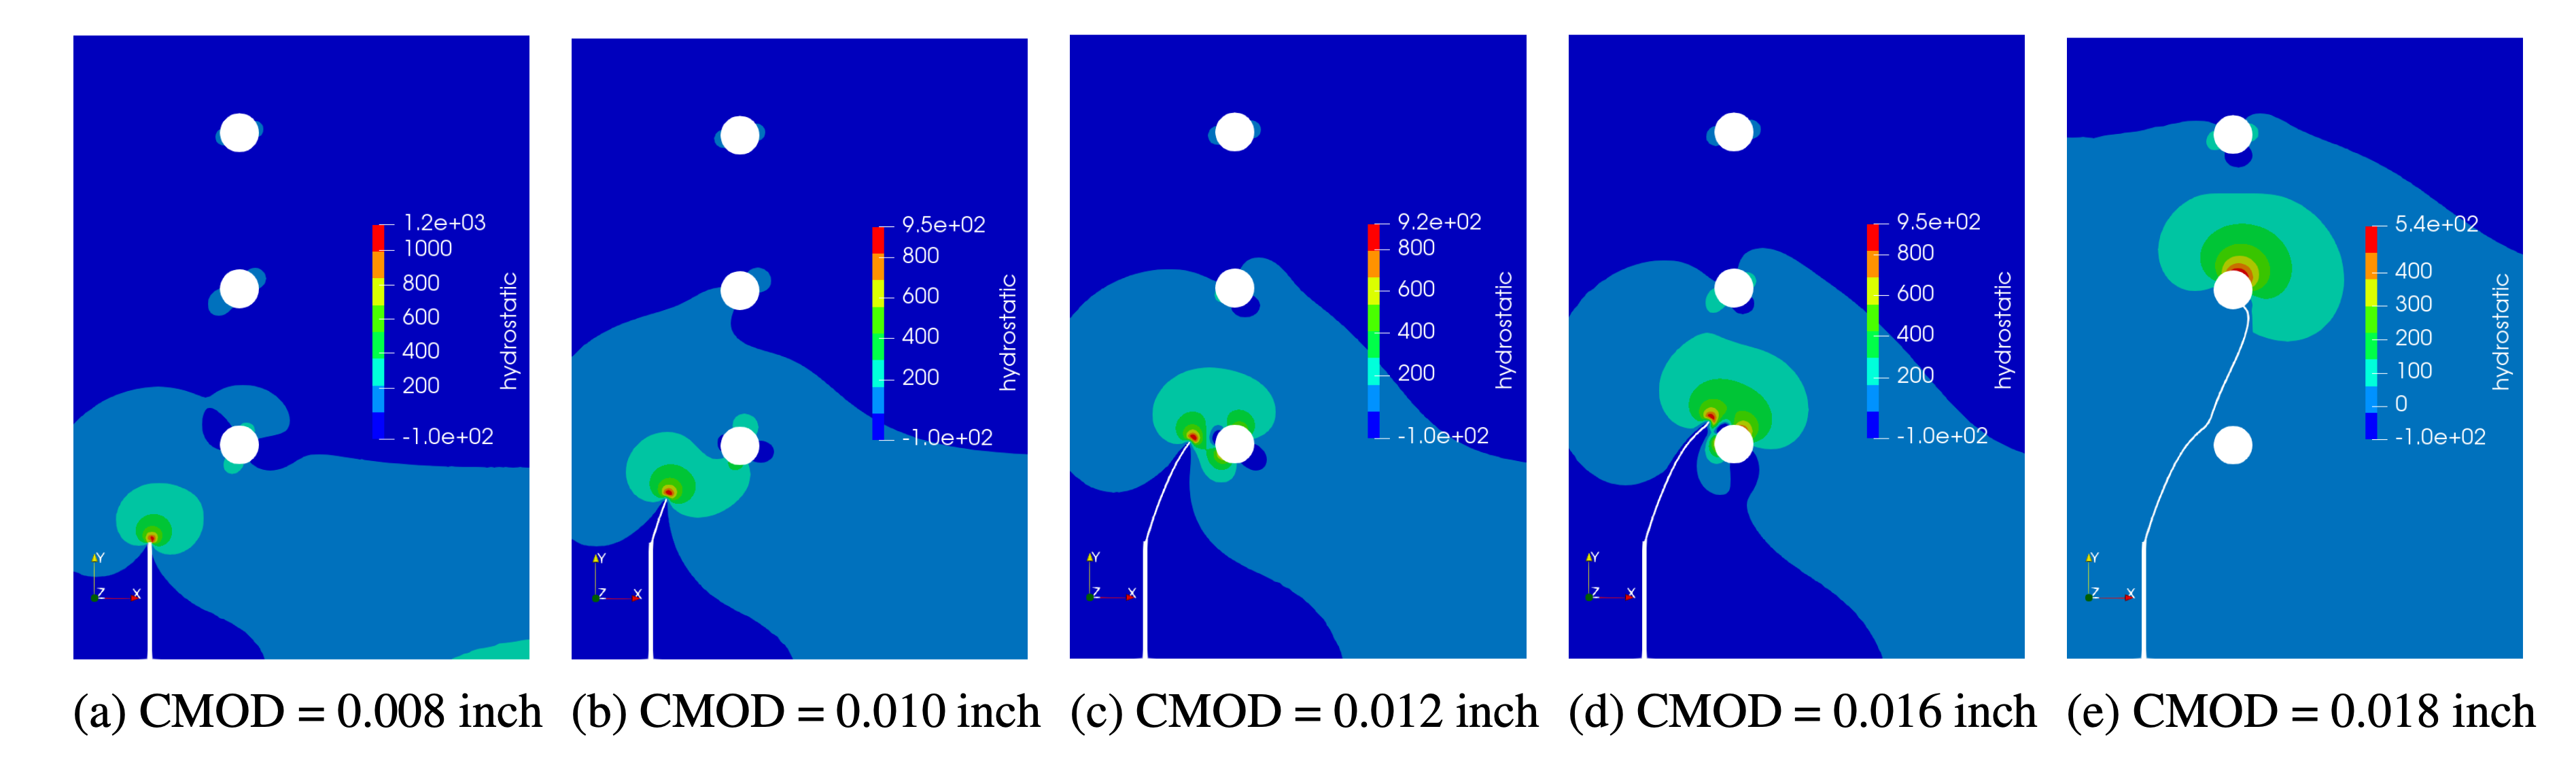
\includegraphics[width=0.9\textwidth]{figures1}
  \caption{Stacking multiple pictures together with sub-captions using the package \texttt{subfig}.}
  \label{fig:figures1}
\end{figure}

%---------------------------------------------------------------------------
\begin{figure*}[!h]
  \begin{snippetlatex}[caption={Stacking multiple images using \LaTeX\ package \texttt{subfig}.},label={snippet_sub_figures},framerule=1pt,tabsize=3]
    \begin{figure}[h!] \centering
    \subfloat[CMOD=0.008 inch]{\includegraphics[width=0.18\textwidth]{t4}\label{fig:a}}\;
    \subfloat[CMOD=0.010 inch]{\includegraphics[width=0.18\textwidth]{t6}\label{fig:b}}\;
    \subfloat[CMOD=0.012 inch]{\includegraphics[width=0.18\textwidth]{t0}\label{fig:c}}\;
    \subfloat[CMOD=0.016 inch]{\includegraphics[width=0.18\textwidth]{t8}\label{fig:d}}\;
    \subfloat[CMOD=0.018 inch]{\includegraphics[width=0.18\textwidth]{t3}\label{fig:e}}\;
    \caption{Asymmetric notched beam under three-point bending: crack evolution.}
    \label{fig:bittencourt-evolution}
    \end{figure}
  \end{snippetlatex}
\end{figure*}
%---------------------------------------------------------------------------

\subsubsection{Sketches}\label{sec:sketches}

If you use \texttt{Illustrator} for some drawings and need to include mathematical symbols in them, then try the application called \texttt{LaTeXiT}\footnote{This software can be found at \url{https://www.chachatelier.fr/latexit/}. Note that, it works only for Mac OS.} to typeset whatever symbols and drag and drop them to \texttt{Illustrator} as embedded PDFs\footnote{Presentations can be created using \texttt{Keynotes} with equations created using \texttt{LaTeXiT} in exactly the same way.}.  \cref{fig:figures11a} presents an example. The same thing can be done using \texttt{Inkscape} with some \LaTeX\ extensions. This is achieved by writing all text or formula using \LaTeX\ syntax in \texttt{Inkscape}. For example, if we want to get $\nabla \sigma$, we write the following text in  \texttt{Inkscape}:

\begin{verbatim}
$\nabla \sigma$
\end{verbatim}

Saving the drawing into the SVG format (SVG is short for scalable vector graphic file), and then exporting it as a PDF\_TEX file using the following command (\cite{inkscape})\footnote{This can also be done using the GUI: File/Save as/ and enable the option 'Omit text in PDF and create LaTeX file'.}:
\begin{verbatim}
inkscape -z -D --file=input.svg --export-pdf="output.pdf" --export-latex
\end{verbatim}
This command generates two files: one is \textit{output.pdf} and the other is \textit{output.pdf\_tex}. And 
then we insert the figure using the file \textit{output.pdf\_tex}, see \cref{snippet_latex_figure} (use line 5). \cref{fig:figures11b} presents an example.

Some people even go to the extreme of not using a graphics software with a user interface (e.g. \texttt{Illustrator}). Instead, they use  \texttt{TikZ}, a \LaTeX\ package for creating graphics programmatically. It has a steep learning curve but the results are outstanding. An example is provided in \cref{fig:tikz}. The code used to generate this drawing is given in \cref{snippet_code_tikz}. One can appreciate the fact that it is fully parameterized, \ie the size of the drawing is controlled by the variable $L$.






\begin{figure}[!h]
  \centering
  \subfloat[\texttt{Illustrator} and \texttt{LaTeXiT}]{\includegraphics{Taylor-bar-setup}\label{fig:figures11a}}
  \subfloat[\texttt{Inkscape} and PDF\_TEX]{\input{Taylor-bar-setup_pdf_tex.pdf_tex}\label{fig:figures11b}}
  \caption{Using \texttt{Illustrator} and \texttt{Inskcape} to produce vector images with \LaTeX\ symbols. The font in figure (a) is slightly different from the one in the text ($\nabla\cdot\boldsymbol{\sigma} = \boldsymbol{\mathit{0}}$), while it matches perfectly in figure (b).}
  \label{fig:figures11}
\end{figure}

%---------------------------------------------------------------------------
\begin{figure}[h!]
  \begin{center}
    \input{vertical_bar_geometry_schematic.tex}
    \caption{Example of schematic made using \texttt{TikZ}.}
    \label{fig:tikz}
  \end{center}
\end{figure}

    

\begin{figure*}[!h]
  \begin{snippetlatex}[caption={\texttt{TikZ} code used to obtain \cref{fig:tikz}.},label={snippet_code_tikz},framerule=1pt,tabsize=3]
    \begin{tikzpicture}[darkstyle/.style={circle,draw,fill=gray!40,minimum size=20}]
      \tikzmath{
        \L = 3;
        \h = \L / 30;
      }
      \draw [thick] (-\L/2,-\L/2) rectangle (\L/2,\L/2);
      \draw [thick] (\L/2, -\L/2) -- (\L/2+\L/5, -\L/2+\L/5);
      \draw [thick] (\L/2+\L/5, -\L/2+\L/5) -- (\L/2+\L/5, \L/2+\L/5);
      \draw [thick] (\L/2, \L/2) -- (\L/2+\L/5, \L/2+\L/5);
      \draw [thick] (-\L/2+\L/5, \L/2+\L/5) -- (\L/2+\L/5, \L/2+\L/5);
      \draw [thick] (-\L/2, \L/2) -- (-\L/2+\L/5, \L/2+\L/5);
      \draw [->] (0,0) -- (0,-\L/4);
      \node [right,thick] at (0, -\L/8) {\large $\boldsymbol{g}$};
      \draw [<->] (-\L/2,-\L/2 - \L/8) -- (\L/2,-\L/2 - \L/8);
      \draw [<->] (\L/2,-\L/2 - \L/8) -- (\L/2+\L/5,-\L/2 - \L/8+\L/5);
      \draw [<->] (-\L/2 -\L/8, - \L/2) -- (-\L/2 -\L/8, \L/2);
      \node [anchor=east] at (-\L/2 - \L/8,0) {1};
      \node [anchor=north] at (0,-\L/2 - \L/8) {1};
      \node [anchor=north west] at (\L/2+\L/10,-\L/2 - \L/8+\L/10) {1};
      \draw[] (-\L/10, \L/2 + \L/15) circle (\L/20);
      \draw[] (-\L/5-\L/10, \L/2 + \L/15) circle (\L/20);
      \draw[] (\L/10, \L/2 + \L/15) circle (\L/20);
      \draw[] (\L/5+\L/10, \L/2 + \L/15) circle (\L/20);
      \draw [-, fill=white] (-\L/2,\L/2 + \L/20) -- (\L/2,\L/2 + \L/20) --%
      (\L/2+\L/5,\L/2 + \L/20+\L/5) -- (-\L/2+\L/5,\L/2+\L/20+\L/5)--(-\L/2,\L/2+\L/20);
      \draw [-] (\L/10,\L/2 + \L/20+\L/10) -- (\L/10,\L/2 + 3*\L/10);
      \draw [-] (\L/10-\L/10,\L/2 + 3*\L/10) -- (\L/10+\L/10,\L/2 + 3*\L/10);
      \draw [-] (\L/10-\L/10,\L/2 + 3*\L/10) -- (\L/10-\L/10+\L/20,\L/2+3*\L/10+\L/20);
      \draw [-] (\L/10,\L/2 + 3*\L/10) -- (\L/10 + \L/20,\L/2 + 3*\L/10 + \L/20);
      \draw [-] (\L/10+\L/10,\L/2 + 3*\L/10) -- (\L/10+\L/10+\L/20,\L/2+3*\L/10 +\L/20);
      % Triad:
      \draw [->] (\L/2+\L/5+\L/8,0) -- (\L/2+\L/5+2*\L/8,0);
      \draw [->] (\L/2+\L/5+\L/8,0) -- (\L/2+\L/5+\L/8*0.29,0-0.71*\L/8);
      \draw [->] (\L/2+\L/5+\L/8,0) -- (\L/2+\L/5+\L/8,0+\L/8);
      \node [anchor=north] at (\L/2+\L/5+\L/8*0.29,0-0.71*\L/8) {$x$};
      \node [anchor=south] at (\L/2+\L/5+\L/8,0+\L/8) {$z$};
      \node [anchor=west] at (\L/2+\L/5+2*\L/8,0) {$y$};
      \draw [fill=red, red] (-\L/2,-\L/2) circle (1pt);
    \end{tikzpicture}
  \end{snippetlatex}
\end{figure*}



%---------------------------------------------------------------------------

\subsubsection{Contour plots}\label{sec:contours}

Another type of images in scientific papers is contour plots (see \cref{fig:figures1}), which are the outcomes of some visualization application such as \texttt{ParaView}\footnote{As we embrace as much as possible open source software, we did not mention \texttt{tecplot},  a good data visualization package developed explicitly for engineers and scientist.}. These images should contain a color bar, and color bars limits should be the same on contour plots you are comparing, otherwise it is very difficult to compare. We do not know how to match the font used in these images with the one in the text. We simply save them as PNG files of highest resolution and include them in the \LaTeX\ document in the same manner as PDF images.

For complex drawings we have to combine the different tools together. \cref{fig:complex-fig} shows one example in which we combined \texttt{ParaView}, \texttt{matplotlib} and \texttt{Inkscape}. 



\begin{figure}[h!]
\centering
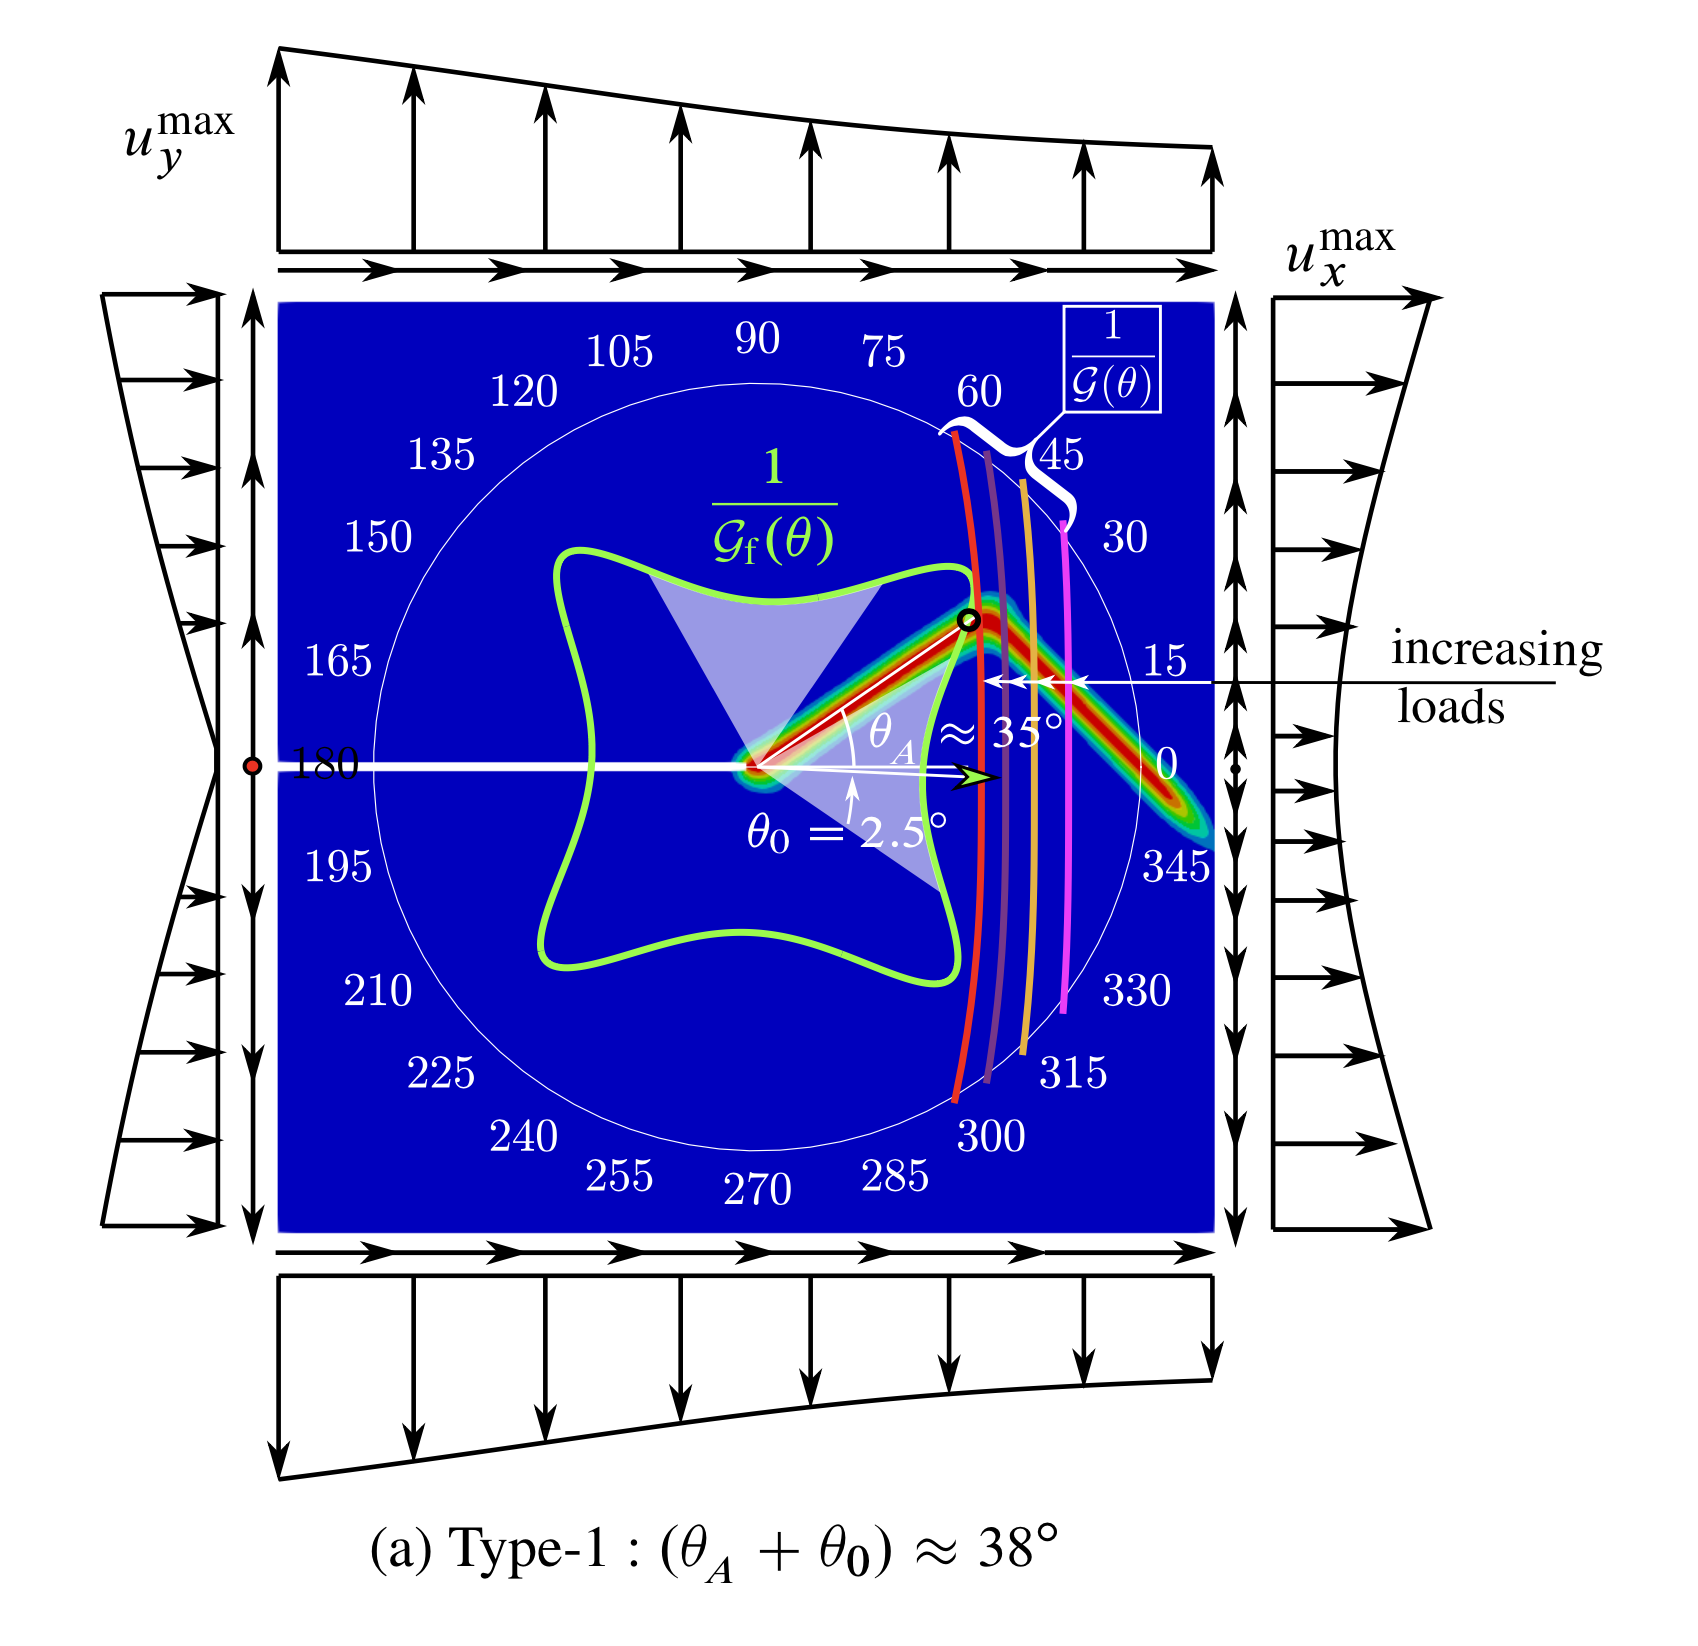
\includegraphics[width=0.4\textwidth]{complex-fig}
\caption{Complex figures: contour plot from \texttt{ParaView} is combined with a polar plot from \texttt{matplotlib} using \texttt{Inkscape}.}
\label{fig:complex-fig}
\end{figure}


 

%--------------------------------------
\subsection{Tables}\label{sec:tabs}

Tables in scientific papers should be clear and focus on the data. Here are some suggestions for making good tables: avoid vertical lines, avoid double horizontal lines, avoid boxing up cells and leave enough space between rows. 
\cref{table:params} satisfies all the criteria. The \LaTeX\ code is shown in \cref{snippet_latex_table}. 
\cref{table:params-foot} in \cref{sec:tab-foonote} presents a table with footnotes.

 \begin{table*}[h!]
      \centering
      \caption{Material parameters and characteristics for all simulations.}
      \setlength\fboxsep{0pt}
      \vskip-\topsep%
      \smallskip%
      \renewcommand\arraystretch{1.4}
      \colorbox{darkgray}{%
      \begin{tabularx}{0.7\textwidth}{lll}
      \toprule
      Parameter                & Section 5.1     & Section 5.2     \\
      \midrule
      Young's modulus [MPa]    & $210\times10^3$ & 145            \\
      Poisson's ratio [-]      & 0.3             & 0.45            \\
      Tensile strength [MPa]   & 2445            & 20              \\
          \midrule 
      Experimentally validated & n/a             & n/a            \\
      Solver                   & multi-step AM   & single-step AM implicit-explicit \\
      State                    & Plane strain    & Plane strain    \\
       \bottomrule
       \end{tabularx}%
      }
      \label{table:params}
      \end{table*}


%---------------------------------------------------------------------------
\begin{figure*}[!h]
  \begin{snippetlatex}[caption={Typesetting tables in \LaTeX. Note that all columns are nicely aligned with \texttt{AlignTab} package in \texttt{Sublime Text}. There exist some software that can convert \texttt{Excel} tables to \LaTeX\ or visually generate \LaTeX\ tables online (\url{https://www.tablesgenerator.com}). Note that the table was shaded with a dark-gray color; it is just a personal taste. Remove lines 8 and 22 will undo this. },label={snippet_latex_table},framerule=1pt,tabsize=3]
    \begin{table}[h!]
    \centering
    \caption{Material parameters and characteristics for all simulations.}
    \setlength\fboxsep{0pt}
    \vskip-\topsep%
    \smallskip%
    \renewcommand\arraystretch{1.4}
    \colorbox{darkgray}{%      
    \begin{tabularx}{0.7\textwidth}{lll}
    \toprule
    Parameter                & Section 5.1     & Section 5.2     \\
    \midrule
    Young's modulus [MPa]    & $210\times10^3$ & 145            \\
    Poisson's ratio [-]      & 0.3             & 0.45            \\
    Tensile strength [MPa]   & 2445            & 20              \\
    \midrule 
    Experimentally validated & n/a             & n/a            \\
    Solver                   & multi-step AM   & single-step AM implicit-explicit \\
    State                    & Plane strain    & Plane strain    \\
    \bottomrule
    \end{tabularx}%
    }
    \label{table:params}
    \end{table}
  \end{snippetlatex}
\end{figure*}
%---------------------------------------------------------------------------

%The angle was \ang{12.3} The brightness was \SI{.23e7}{\candela} \SI{20}{MPa} \SI{10}{N.m.m^{-2}}

If you look at the figures and tables in any paper including this one you will see that figure captions are generally placed below the figures, whereas table captions must be placed above the tables. This is because we generally read tables from the top down, and therefore want to see the caption at the top. Figures are not always read top down. When you open a page and see a figure, the first thing you want to know is “what is that?” The caption below it should immediately identify what the figure represents for the reader.  If you choose to do the opposite \eg placing figure captions above the figures, do so consistently throughout your document.

\subsection{Equations}\label{sec:equation-latex}


With \latex it is possible to get nice mathematical symbols and equations, for example

\begin{equation}
  \mathscr{E} (\bfu, d) 
    = \int_{\varOmega_{0}} \left[\omega(d)\psi_{0}^+(\bfepsilon (\bfu)) + \psi_{0}^-(\bfepsilon (\bfu)) \right]\td V
    + \int_{\varOmega_{0}}  \frac{G_\text{f}}{c_\alpha} \left[ \frac{1}{b} \alpha(d)
    + b \left( \nabla d \cdot \nabla d \right) \right] \td V
    - \mathscr{P} (\bfu)   
\label{eq:3}
\end{equation}
The \LaTeX\ code used to generate this equation is given in \cref{snippet_latex_eq}. To speed up the typing of commonly used symbols, they have been redefined (\ie made short) and put in a .tex file (see pre\_commands.tex in \cref{snippet_template}). You can check this file at our github repository to know how to define a new command.

For more details on how to typeset formulas in \LaTeX\, see chapter 3 of \cite{latex}. To be self-containing, \cref{sec:writing_equation} discusses how to write complex equations.

%---------------------------------------------------------------------------
\begin{figure*}
  \begin{snippetlatex}[caption={\LaTeX\ commands to generate \cref{eq:3}. Each equation should have a unique label.},label={snippet_latex_eq},framerule=1pt,tabsize=3]
    \begin{equation}
      \mathscr{E} (\bfu, d) 
        = \int_{\varOmega_{0}} \left[\omega(d)\psi_{0}^+(\bfepsilon (\bfu)) + 
        \psi_{0}^-(\bfepsilon (\bfu)) \right]\td V + 
        \int_{\varOmega_{0}}  \frac{G_\text{f}}{c_\alpha} \left[ \frac{1}{b} \alpha(d)
        + b \left( \nabla d \cdot \nabla d \right) \right] \td V
        - \mathscr{P} (\bfu)   
    \label{eq:3}    % use this label 'eq:3' in \cref{eq:3} to refer to this in text
    \end{equation}
  \end{snippetlatex}
\end{figure*}
%---------------------------------------------------------------------------





\subsection{Algorithm}\label{sec:algorithm}

The packages \texttt{algorithm} and \texttt{algorithmicx} can be used to typeset algorithms. See  \cref{alg:alg10-a} for an example. These algorithms written as pseudo codes are easier to understand than flowcharts. Yet, they are also easier to generate, directly with \LaTeX. We refer to our github repository for the source.

\begin{center}
\setlength\fboxsep{0pt}
\vskip-\lastskip%
%\smallskip%
\colorbox{darkgray}{%
%\graybox{
\begin{minipage}{\linewidth}
\vspace{-12pt}
      \begin{algorithm}[H]
        %\small
        \caption{Stress update algorithm.} % give the algorithm a caption
        \label{alg:alg10-a} 
        \begin{algorithmic}[1] % enter the algorithmic environment
          \State Inputs: $\varepsilon_p^t$ (equivalent plastic strain), $\bsym{\sigma}^{\prime~d}_{t}$ (un-rotated deviatoric stress), $\vm{d}^d$, damage $D^t$
          \State Outputs: $\varepsilon_p^{t+\Delta t}$ (equivalent plastic strain), $\bsym{\sigma}^{\prime~d}_{t+\Delta t}$
          \State Compute $G'=(1-D^t)G$
          \State $\bsym{\sigma}^{\prime~d}_\text{trial} = \bsym{\sigma}^{\prime~d}_{t} + 2G'\Delta t \vm{d}^d$\Comment{purely elastic stress deviator update}
          \State $\sigma^{\prime~\text{eq}}_\text{trial} = \sqrt{\frac{3}{2} \bsym{\sigma}^{\prime~d}_\text{trial}:\bsym{\sigma}^{\prime~d}_\text{trial}}$\Comment{equivalent von Mises trial stress}
          \State $\sigma_f = \left[A+B\left(\varepsilon_p^t\right)^n\right]\left[1+C\ln\dot{\varepsilon}_p^*\right] \left[ 1 - (T^\ast)^m \right]  (1-D^t)$\Comment{JC flow stress}
          \If{$\sigma_\text{trial}^{\prime~\text{eq}} < \sigma_f$} \Comment{yielding did not occur, purely elastic step}
          \State $\bsym{\sigma}^{\prime~d}_{n+1} = \bsym{\sigma}^{\prime~d}_\text{trial}$ \Comment{keep trial deviatoric stress}
          \Else \Comment{yielding has occurred}
          \State $\Delta \varepsilon_{p} = (\sigma^{\prime~\text{eq}}_\text{trial} - \sigma_{f})/ (3G')$ \Comment{compute the equivalent plastic strain increment}
          \State $\varepsilon^{t+\Delta t}_p = \varepsilon^{t}_p + \Delta \varepsilon_{p}$\Comment{update the undamaged matrix plastic strain}
          \State $\bsym{\sigma}^{\prime~d}_{t+\Delta t} = \frac{\sigma_{f}}{\sigma^{\prime~\text{eq}}_\text{trial}} \bsym{\sigma}^{\prime~d}_\text{trial}$ \Comment{scale deviatoric stress back to yield surface}
          \EndIf
        \end{algorithmic}
      \end{algorithm}
      %\vspace{-10pt}
      \end{minipage}%
      }
\end{center}

%------------------------------------------------
\subsection{Source code}\label{sec:source-code}

Source code can be included in \LaTeX\ using either the \texttt{Listing} package or the \texttt{minted} package. As the installation of the latter package is more involved (it requires an external program), we present in \cref{list-array} some C++ source code using the \texttt{Listing} package which does not depend on external program. We refer to the \LaTeX\ source of this paper for the configuration of this package to produce \cref{list-array}.

% ----------------------------------------------------------------
\begin{code-c-num}[caption={Presentation of source code using the \texttt{Listing} package with the Bera Mono font (\url{https://tug.org/FontCatalogue/beramono/}). },
                   label={list-array},framerule=1pt]
    #include <jive/Array.h>
    #include <jem/base/System.h>
    using jive::Vector;    
    using jive::Matrix;
    
    Vector      a;             // double vector Array<double>
    Matrix      A(10,20);      // double matrix Array<double,2>

    A(slice(BEGIN,3),2) = 2.0; // third col, rows 0, 1, 2 = 2
    System::out() << A << "\n";// similar to std::cout << A << "\n";
\end{code-c-num}
% ----------------------------------------------------------------

%--------------------------------
\subsection{Two-column format}\label{sec:two-col}

Preparing two-column papers is harder than one-column papers. \cref{snippet_two_cols} presents \LaTeX\ snippets for long figures, tables and equations that span the whole width of the paper. That's all \LaTeX\ can do for you. For equations that are just a bit longer than one column, you have to manually modify them to make them fit.

%---------------------------------------------------------------------------
\begin{figure*}[!h]
  \begin{snippetlatex}[caption={Writing two-column papers using \LaTeX.},label={snippet_two_cols},framerule=1pt,tabsize=3]
    \usepackage{mathtools, cuted} % 2 colum format, long equation

     % big figure span the whole page
    \begin{figure*}[!h]
    \end{figure*}

    % big table span the whole page
    \begin{table*}[!h]
    \end{table*}
   
     % using strip for long equations
    \begin{strip}
     % put your long equation here
    \end{strip}
  \end{snippetlatex}
\end{figure*}
%---------------------------------------------------------------------------

At this stage you know how to use \LaTeX, to write a high quality technical paper and you have just completed one such paper. Is it ready for submission? The next section provides some steps taken to answer this question. 


%%%%%%%%%%%%%%%%%%%%%%%%%%%%%%%
\section{Submission}\label{sec:submission}

Do not submit until you are really happy with the work, as it usually does not save time to submit a piece of work which we know ourselves could be improved: the reviewers will think likewise, or be even more critical than we are ourselves of our work. If on a final read of the paper you think: “Ah… I could have added this study. This argument is not completely convincing to me. This graph could be better plotted. I think I forgot some relevant literature. The notations are complex, perhaps the reader will have difficulties…” Then, do not submit immediately, improve your work, and submit it when it is ready. 

It is also useful to ask peers to read over your work. Before giving your first draft to your supervisor(s), have it proof-read by a peer (\ie if you are a PhD student, ask another PhD student for their opinion). This will bring the following positive points: 
It will value your peer as you think her/his opinion counts;
It will give you insights on how understandable your paper is by someone who is connected to your field but did not do exactly the same piece of research;
It will decrease the number of typos, which will enable your supervisor(s) to focus on the scientific content as opposed to bumping over each spelling mistake, grammatical error, jargon. 

It is most effective to get feedback sequentially rather than in parallel. For example, rather than asking four people to read the same version of your paper, ask one person to read the paper, then make revisions before asking the next person to read it, and so on. This prevents you from getting the same comments repeatedly.

Now you have submitted our paper and gotten the reviews back, and the editor has asked you to revise your paper taking into account the reviewers' comments. How should you tackle this task? Different people have different ideas but you can start with \cite{noble2017ten} if you do not know where to begin.

%%%%%%%%%%%%%%%%%%%%%%%%%%%%%%%
\section{Conclusions}

Does this paper really need a conclusion section? Not really, but we are a bit conservative. So, here you are. Without claiming  originality of ideas presented in this short paper, we have presented a collection of  suggestions and recommendations that can streamline the writing process. Following them would result in readable scientific articles which in turn save time for the authors,  the editors, the reviewers and the readers.


As \LaTeX\ and the tools we are relying on keep evolving, we will constantly update this article to reflect changes. The updated version of this paper and scripts can be obtained at the github account of the first author (\url{https://github.com/vinhphunguyen/how-to-write-a-paper}).

Our guidelines are rules not principles. Unlike principles, rules break all the time. Feel free to be creative as long as you write to inform not to impress. Happy writing.

%
%%%%%%%%%%%%%%%%%%%%%%%%%%%%%%%
\section*{Acknowledgments}

 The first author (V.P. Nguyen) thanks the funding support from the Australian Research Council via DECRA project DE160100577.  The third  author gratefully acknowledges the financial support of the Australian Research Council (ARC) Training Centre in Alloy Innovation for Mining Efficiency (IC160100036).

 The guidelines presented in this paper have been formed by reading many articles and books and learning from them. Our favorite author is Ted Belytschko. We have also learned a lot through interactions with our co-authors. In particular, we would like to thank L. J. Sluys and M. Stroeven (TU Delft, the Netherlands), and Chad W. Sinclair (UBC, Canada).



%% The Appendices part is started with the command \appendix;
%% appendix sections are then done as normal sections
%=============================================================================
\begin{appendices}
%=============================================================================
%\showthe\textwidth % => width of the pdf, see in log file, is 468 pt. use it in plot.py for great plots.
%
\crefalias{section}{appsec}

%-------------------------------
\section{Installing \LaTeX}\label{sec:latex-installation}

To help those new to \LaTeX\, herein we present how to set up \LaTeX\ for  macOS and Ubuntu computers, the operating systems that we use.

For macOS, do the following
\begin{enumerate}
    \item Install \texttt{macTeX} from \url{http://www.tug.org/mactex/}
     \item It comes with \texttt{TexShop}--a LaTeX editor, so you can start using \LaTeX\ immediately.
\item To get the pdf of this paper, open TexShop (in folder /Applications/TeX/), press Command T, and you're done. 
\item If you want to use \texttt{Sublime Text}, check \href{http://individual.utoronto.ca/dobronyi/latexsublime.html}{this blog}.
\end{enumerate}
And for Ubuntu,
\begin{enumerate}
    \item Install \texttt{Tex Live}: sudo apt-get install texlive-full
\item Install a Tex editor, for example, \texttt{TexMaker}: sudo apt-get install texmaker
\item How to use \texttt{TexMaker}: \url{https://www.xm1math.net/texmaker/}.
\item For \texttt{emacs}, check \href{https://www.wangzerui.com/2017/02/21/setting-up-a-nice-environment-for-latex-on-ubuntu/}{this blog}.
\end{enumerate}

\section{Python scripts for plotting data}\label{sec:scripts}

This appendix present two \texttt{Python} scripts to produce high quality graphs which have the same font used in the paper. One can use the script shown in \cref{snippet_matplotlib} to get PDFs or the one in \cref{snippet_matplotlib_pgf} to get PGF files. PGF pictures can be embedded as raw commands in \LaTeX\ documents. The original source is \url{https://jwalton.info/Embed-Publication-Matplotlib-Latex/}.

The main idea is to get the correct figure size, and insert it in the paper without scaling. To determine the figure size, one first calculates the width of the paper, which can be done by inserting this command in the \LaTeX\ file:


\begin{verbatim}
\showthe\textwidth % => width of the pdf, see in log file, is 468 pt. 
\end{verbatim}
Then you can search for `width of the pdf' in this log file to find out the width of your paper.

\begin{figure*}[!h]
  \begin{snippet}[caption={Python script for plotting data (PDF).},label={snippet_matplotlib},framerule=1pt,tabsize=3]   
    import matplotlib as mpl
    import matplotlib.pyplot as plt
    def set_size(width, fraction=1, subplot=[1, 1]):
        if width == 'elsevier':
            width_pt = 468.
        elif width == 'beamer':
            width_pt = 307.28987
        else:
            width_pt = width
        fig_width_pt = width_pt * fraction      # Width of figure
        inches_per_pt = 1 / 72.27               # Convert from pt to inches
        golden_ratio = 0.75                     # (5**.5 - 1) / 2
        fig_width_in = fig_width_pt * inches_per_pt  # Figure width in inches
        fig_height_in = fig_width_in * golden_ratio * (subplot[0] / subplot[1])
        fig_dim = (fig_width_in, fig_height_in)
        return fig_dim
    parser = argparse.ArgumentParser(description='Plot the evolution of variables.',
                                     add_help=False,
                                     formatter_class=argparse.RawDescriptionHelpFormatter)

    parser.add_argument('--quiet', '-q', action='store_const', const=True, default=False,
                        help='do not show plot.')
    args = parser.parse_args()
    plt.style.use('seaborn-colorblind')      # Using seaborn's style
    nice_fonts = {
            "text.usetex": True,
            "font.family": "serif",
            "axes.labelsize": 10,
            "font.size": 10,
            "legend.fontsize": 8,
            "xtick.labelsize": 8,
            "ytick.labelsize": 8,
    }
    mpl.rcParams.update(nice_fonts)
    # Dimer 5: Read Data
    fnames = ['log.mpm', 'dam-break-Sun.csv', 'water-break-experiment.csv']
    dat    = [pylab.genfromtxt(f,skip_header=1) for f in fnames]
    fig, ax = plt.subplots(1, 1, figsize=set_size('elsevier', fraction=0.6))
    # fig, (ax1,ax2) = plt.subplots(1, 2, figsize=set_size(width, subplot=[1, 2]))
    for i, f in enumerate(fnames):   
        x = dat[i][:,3]
        y = dat[i][:,4]
        ax.plot(x, y, color='black', label='MPM',linewidth=1.5, linestyle='dotted')
        xmax = max(xmax, np.max(x))
        ymax = max(ymax, np.max(y))
        ax.set_xlabel(r'$T$')
        ax.set_ylabel(r'$L(T)$')
        ax.set_ylim(1.0, 2.8)
        ax.set_xlim(0, 1.6)
        ax.legend(loc=0)
        plt.tight_layout()
        plt.savefig('./water-break-plot.pdf', format='pdf', bbox_inches='tight')
        if args.quiet == False:
            plt.show()
  \end{snippet}
\end{figure*}

\begin{figure*}[!h]
  \begin{snippet}[caption={Python script for plotting data (PGF).},label={snippet_matplotlib_pgf},framerule=1pt,tabsize=3]   
    nice_fonts = {
            "text.usetex": True,
            "font.family": "serif",
            "pgf.texsystem": "pdflatex",
            "font.family": "serif",
            "font.serif": [],
            "font.sans-serif": [],
            "font.monospace": [],
            "pgf.preamble": [
            # put LaTeX preamble declarations here
            r"\usepackage[utf8x]{inputenc}",
            r"\usepackage[T1]{fontenc}",
            # macros defined here will be available in plots, e.g.:
            r"\newcommand{\vect}[1]{#1}",
            # You can use dummy implementations, since you LaTeX document
            # will render these properly, anyway.
            ],
            "axes.labelsize": 10,
            "font.size": 10,
            "legend.fontsize": 8,
            "xtick.labelsize": 8,
            "ytick.labelsize": 8,
    }
    plt.savefig('./cold-spray-plots.pgf', bbox_inches='tight') 
    if args.quiet == False:
        plt.show()
  \end{snippet}
\end{figure*}

\begin{rmk}
If you are using \texttt{Matlab}, then try this script \texttt{matlab2tikz} for converting \texttt{Matlab} figures into native TikZ/Pgfplots figures. The script can be found at
\url{https://www.mathworks.com/matlabcentral/fileexchange/22022-matlab2tikz-matlab2tikz}.
\end{rmk}

%-------------------------------
\section{Tables with footnotes}\label{sec:tab-foonote}

Making tables with footnotes in \LaTeX\ is not straightforward.  \cref{table:params-foot} is one example and we refer to the source (at our github account) to see how it was made. It is probably not an elegant solution but it is the best solution we have found.

\begin{table*}[!h]
      \centering
      \caption{A table with footnotes generated using package \texttt{threeparttable}.}
      \label{table:params-foot}
      \setlength\fboxsep{0pt}
      \vskip-\topsep%
      \smallskip%
      \renewcommand\arraystretch{1.4}
      \begin{threeparttable}
      \centering
      \colorbox{darkgray}{%
      \begin{tabularx}{0.9\textwidth}{lll}
      \toprule
      Parameter                & Section 5.1     & Section 5.2     \\
      \midrule
      Young's modulus [MPa]    & $210\times10^3$ & 145\tnote{\textdagger}            \\
      Poisson's ratio [-]      & 0.3             & 0.45            \\
      Tensile strength [MPa]   & 2445            & 20\tnote{\ddag}              \\
          \midrule 
      Experimentally validated & n/a             & n/a            \\
      Solver                   & multi-step AM   & single-step AM implicit-explicit \\
      State                    & Plane strain    & Plane strain    \\
       \bottomrule
       \end{tabularx}%
      }
      \parbox{\linewidth}{
      \begin{tablenotes}[flushleft]
      \footnotesize
      \item[\textdagger] Footnote1
      \item[\ddag]Taken from \cite{Mandal:EFM2019}.
    \end{tablenotes}}
    \end{threeparttable}
      \end{table*}




%-------------------------------
\section{Reference management with \texttt{BibDesk}}\label{sec:bibdesk}
 

This section presents some ideas on how we manage our library (bibliography entries plus the associated PDFs) using \texttt{BibDesk}. The original source is \url{https://atchieu.wordpress.com} (search for \texttt{BibDesk}). 

We have a single \texttt{.bib} file for our library. This file is stored in a \texttt{Dropbox} folder so that it syncs to all devices. \texttt{BibDesk} is configured such that whenever a PDF is added to a 
bibliography entry, the PDF will be automatically renamed and stored in a specified location (in \texttt{Dropbox}) with a specified file naming convention. You do not  care where they go: just go to \texttt{BibDesk} and search for the article and the PDF is there.

\section{Writing equations} % (fold)
\label{sec:writing_equation}

This appendix presents some equations that are hard to create using \LaTeX\ for beginners. 

For example, to get the following equation, 

\begin{equation}
\begin{array}{ll}
  \dfrac{D \rho}{Dt} + \rho \nabla \cdot \vm{v} = 0 & \text{(conservation of mass)}\\[8pt]
\rho\dfrac{D\vm{v}}{Dt}  = \nabla \cdot \bsym{\sigma} + \rho \vm{b}
& \text{(conservation of linear momentum)} \\[8pt]
  \rho \dfrac{D e}{Dt}  = \vm{D}:\bsym{\sigma}   & \text{(conservation of energy)}\\[8pt]
   \vm{v}(\vm{x},t=0) = \vm{v}_0,\; \bsym{\sigma}(\vm{x},t=0) = \bsym{\sigma}_0
   & \text{(initial conditions)}
   \label{eq:governing}
\end{array}
\end{equation}
we use an \texttt{array} inside an \texttt{equation} block (\cref{snippet_strong_form}). This way produces only one number for the entire equation only.


%---------------------------------------------------------------------------
\begin{figure*}[!h]
  \begin{snippetlatex}[caption={Writing \cref{eq:governing} using \LaTeX.},label={snippet_strong_form},framerule=1pt,tabsize=3]
    \begin{equation}
    \begin{array}{ll}
      \dfrac{D \rho}{Dt} + \rho \nabla \cdot \vm{v}=0&\text{(mass conservation)}\\[8pt]
    \rho\dfrac{D\vm{v}}{Dt}  = \nabla \cdot \bsym{\sigma} + \rho \vm{b}
    & \text{(conservation of linear momentum)} \\[8pt]
      \rho \dfrac{D e}{Dt}  = \vm{D}:\bsym{\sigma}&\text{(energy conservation)}\\[8pt]
       \vm{v}(\vm{x},t=0) = \vm{v}_0,\; \bsym{\sigma}(\vm{x},t=0) = \bsym{\sigma}_0
       &  \text{(initial conditions)}
    \label{eq:governing}
    \end{array}
    \end{equation}  
  \end{snippetlatex}
\end{figure*}
%---------------------------------------------------------------------------  



If you want to have labels for all the sub-equations, for example, as in the following equation

\begin{subequations}\label{eq:pfms}
  \begin{IEEEeqnarray}{lll}
  \texttt{Model1}: \quad \alpha(d) = 9d,     \quad & \chi_2 = 0,           \quad & \chi_4 = 1\label{eq:s1}\\
  \texttt{Model2}: \quad \alpha(d) = d^2, \quad & \chi_2 = 1, \quad & \chi_4 = 2
  \end{IEEEeqnarray}
\end{subequations}
you can use \texttt{subequations} and \texttt{IEEEeqnarray} as shown in \cref{snippet_eqnarray}. Each sub-equation has its own label, and thus can be referred to.


%---------------------------------------------------------------------------
\begin{figure*}[!h]
  \begin{snippetlatex}[caption={Writing \cref{eq:pfms} using \LaTeX.},label={snippet_eqnarray},framerule=1pt,tabsize=3]
    \usepackage[retainorgcmds]{IEEEtrantools} % to use IEEEeqnarray
    \begin{subequations}\label{eq:pfms}
    \begin{IEEEeqnarray}{lll}
     \texttt{Model1}:\quad\alpha(d)=9d,\quad & \chi_2=0,\quad&\chi_4=1\label{eq:s1}\\
     \texttt{Model2}:\quad\alpha(d)=d^2,\quad& \chi_2=1,\quad&\chi_4=2\label{eq:s2}
    \end{IEEEeqnarray}
    \end{subequations}
  \end{snippetlatex}
\end{figure*}
%---------------------------------------------------------------------------  



% section writing_equation (end)

\end{appendices}


%%%%%%%%%%%%%%%%%%%%%%%%
%\section*{References}


% %%%%%%% BIB files (bibtex)
%\bibliographystyle{plainnat}
\bibliographystyle{abbrvnat} % => just V. P. Nguyen, not Phu Nguyen, ...
%\bibliographystyle{natbib}
\bibliography{writing}

% if biblatex is used
%\printbibliography

\end{document}

%%% Local Variables:
%%% mode: latex
%%% TeX-master: t
%%% End:
